



%----------------------------------------------------------------------------------------

\newpage

%\section[Interaction model][Modèle d'interaction]{Dynamical extension of the interaction model}{Extension dynamique du modèle d'interaction}
\section{Dynamical extension of the interaction model}{Extension dynamique du modèle d'interaction}



\label{sec:macrocoevol}



%----------------------------------------------------------------------------------------


Nous pouvons à présent étendre la logique d'intégration d'un système de ville et du réseau de transport, effectuée de manière statique pour le comportement du réseau dans le modèle d'interaction développé et exploré en section~\ref{sec:interactiongibrat}, pour proposer une formulation d'un \emph{modèle de co-évolution macroscopique pour les systèmes de villes}.



%%%%%%%%%%%%%%%%%
\subsection{Macroscopic Model of Co-evolution}{Modèle macroscopique de co-évolution}


%%%%%%%%%%%%%%%%%
\subsubsection{Rationale}{Hypothèses et choix de modélisation}



\bpar{
In a multi-modeling fashion, the model can take into account various processes such as between cities direct interactions, network-mediated interactions, feedback of network flows, and for the network demand-induced growth.
}{
Cette première approche se place dans une logique d'extension directe du modèle d'interactions au sein d'un système de villes présenté en chapitre~\ref{ch:evolutiveurban}, c'est-à-dire à une échelle macroscopique et avec une ontologie typique aux systèmes de villes. Toujours dans un choix de simplicité, nous gardons ici une description unidimensionnelle des villes par leur population.

Concernant la croissance du réseau, nous proposons de nous placer également à un niveau relativement agrégé et simplifié, en permettant de tester des heuristiques de croissance à différents niveaux d'abstraction. Dans une logique de flexibilité des mécanismes du modèle, il peut prendre en compte divers processus comme les interactions directes entre les villes, les interactions intermédiaires par le réseau, la rétroaction des flux de réseau et une croissance du réseau induite par la demande.

Les éléments empiriques mis en valeur pour le réseau ferré français par~\cite{thevenin2013mapping} suggèrent l'existence de rétroactions de l'utilisation du réseau, ou des flux le traversant, sur sa persistence et son développement, dont les propriétés ont évolué dans le temps : une première phase de développement fort correspondrait à la réponse du réseau à une demande de forte couverture, suivie d'une phase de renforcement des liens principaux et la disparition des liens les plus faibles.
}

Le couplage entre réseau et ville sera fait par l'intermédiaire des flux entre villes dans le réseau : ceux-ci portent les interactions entre villes et ont simultanément une influence sur le réseau dans lequel ils circulent.



%%%%%%%%%%%%%%%%%
\subsubsection{General Formulation}{Formulation générique}



%%%%%%%%%%%%%%%%%
\begin{figure}
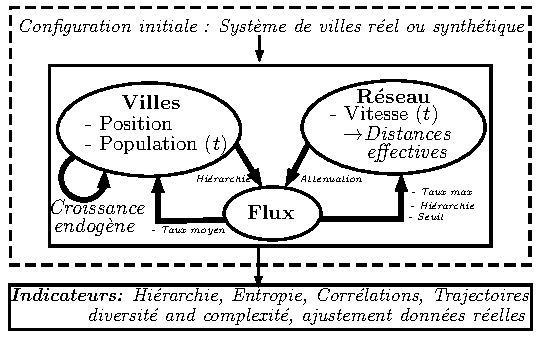
\includegraphics[width=\linewidth]{Figures/MacroCoEvol/model}
\caption[Schematic Model Representation][Schématisation du modèle de co-évolution macroscopique]{\textbf{Abstract representation of the model.}}{\textbf{Représentation abstraite du modèle.} Les ovales correspondent aux éléments ontologiques principaux (Villes, Réseau, Flux), tandis que les flèches traduisent des processus et les paramètres associés sont indiqués. Le modèle est décrit dans son écosystème plus large d'initialisation et d'indicateurs de sortie.\label{fig:macrocoevol:model}}
\end{figure}
%%%%%%%%%%%%%%%%%



Le système urbain est caractérisé par les populations $\mu_i(t)$ et le réseau $\mathbf{G}(t)$ auquel on peut associer une matrice de distance $d^G_{ij}(t)$. Les flux entre villes $\phi_{ij}$ suivent les expressions données en~\ref{sec:interactiongibrat} avec la distance réseau. De la même manière, la variation des populations suit les spécifications du modèle de base. La Fig.~\ref{fig:macrocoevol:model} exprime le modèle sous forme schématisée.




\paragraph{Network Growth}{Croissance du réseau}


Concernant le réseau, nous faisons l'hypothèse que celui-ci évolue suivant
\begin{equation}
\mathbf{G}(t + 1) = F(\mathbf{G}(t),\phi_{ij}(t))
\end{equation}
de telle façon qu'une assignation des flux dans le réseau ainsi qu'une variation locale de ses éléments est possible. Nous proposons dans un premier temps de nous intéresser aux motifs liés à la distance uniquement, et de spécifier une relation sur un réseau abstrait par
\begin{equation}
d^G_{ij}(t+1) = F(d^G_{ij}(t),\phi_{ij}(t))
\end{equation}
c'est-à-dire une évolution de la matrice de distance uniquement. Dans cette logique, nous restons dans un modèle d'interaction à l'échelle strictement macroscopique, puisqu'une spatialisation précise du réseau impliquerait la prise en compte d'une échelle plus fine qui comporte la forme locale du réseau déterminante des plus court chemins.

Suivant l'heuristique de rétroaction par seuil, étant donné un flux $\phi$ dans un lien, on suppose que sa distance effective est mise à jour par :

\begin{equation}
d(t+1) = d(t)\cdot \left( 1 + g_{max} \cdot \left[\frac{1 - \left(\frac{\phi}{\phi_0}\right)^{\gamma_s}}{1 + \left(\frac{\phi}{\phi_0}\right)^{\gamma_s}}\right]\right)
\end{equation}


avec $\gamma_s$ un paramètre de hiérarchie, $\phi_0$ le paramètre de seuil et $g_{max}$ le taux de croissance maximal à chaque étape. Cette fonction d'auto-renforcement s'interprète de la façon suivante : au dessus d'un flux limite $\phi_0$, les conditions de trajet s'améliorent, tandis qu'elles diminuent en dessous. La hiérarchie du gain est donnée par $\gamma_s$ et comme $\frac{1 - \left(\frac{\phi}{\phi_0}\right)^{\gamma_s}}{1 + \left(\frac{\phi}{\phi_0}\right)^{\gamma_s}} \rightarrow_{\phi\rightarrow \infty} -1$, $g_{max}$ est le gain de distance maximal. Il s'agit d'une fonction similaire à celle utilisée par \cite{tero2007mathematical}\footnote{Qui utilise $\Delta d = \Delta t \left[ \frac{\phi^\gamma}{1 + \phi^\gamma} - d\right]$. Cette fonction permet également un effet de seuil, puisque la dérivée s'annule en $\phi^{\ast} = \left(\frac{d}{1 - d}\right)^{1/\gamma}$, mais celui-ci ne peut pas être ajusté.}.

%qui peut s'ajuster à des valeurs réalistes par exemple par l'intermédiaire du calcul de $(1+g_{max})^{t_f}$.\comment[FL]{phrase tres floue}

%cf Tero ? papier Francois \cite{2013arXiv1301.6628K}
% implementation
% https://github.com/fqueyroi/tulip_plugins/tree/master/TransportationNetworks



\subsubsection{Implementation}{Implémentation}



\bpar{
}{
Le couplage du modèle d'interaction à une explicitation du réseau plus fine (par exemple encodage de l'ensemble de la structure du réseau) rend plus difficile l'intégration complète dans un plugin OpenMole comme c'était le cas pour le modèle étudié en~\ref{sec:interactiongibrat}, nécessitant une implémentation \emph{ad hoc}. L'utilisation d'un workflow comme médiateur pour le couplage est une solution intéressante mais réaliste uniquement dans le cas d'un couplage faible comme en~\ref{sec:correlatedsyntheticdata}. L'un des défis que devra relever la bibliothèque de méta-modélisation en cours de développement autour d'OpenMole, est la possibilité de coupler fortement (par exemple au sens de dynamiquement dans l'évolution de la simulation) des composantes hétérogènes de manière transparente, permettant de tirer parti des avantages de différents langages ou d'implémentations déjà existantes.
}

% rq : // idee de Romain stopper dynamiquement les simulations.

\bpar{}{
Nous optons ici pour une implémentation complète en NetLogo pour une simplicité de couplage des composantes. Une attention particulière est portée à la dualité de la représentation du réseau, à la fois sous forme de matrice de distance et sous forme physique, pour permettre facilement l'extension à des heuristiques de réseau physique.
}






%%%%%%%%%%%%%%%%%
\subsection{Application to Synthetic Data}{Application à des données synthétiques}


\bpar{
The model is first tested and explored on synthetic city systems, generated following a simple heuristic to follow the rank-size law and Central Place Theory.
%The systematic exploration through intensive computation unveils different interaction regimes across the parameter space. In some, the introduction of the network can drastically change the fate of some cities, whereas the top-distribution hierarchy is reinforced, what is consistent with empirical observations in the literature. Some regimes suggest circular causalities between network and city growth, corresponding to the co-evolution.
}{
Le modèle est d'abord testé et exploré sur des systèmes de villes synthétiques, afin de comprendre certaines de ses propriétés intrinsèques. Dans ce cas, nous considérons le modèle avec réseau abstrait comme spécifié ci-dessus, c'est-à-dire sans explicitation spatiale du réseau et avec les règles d'évolution agissant directement sur $d^G_{ij}$ selon les spécifications données précédemment.
}


\subsubsection{Synthetic data}{Données synthétiques}


Un système de villes synthétiques est généré, en suivant l'heuristique utilisée dans la section précédente : (i) des villes en nombre $N_S$ sont placées aléatoirement dans le plan euclidien ; (ii) les populations sont attribuées aux villes selon une loi de puissance inverse, avec un paramètre de hiérarchie $\alpha_S$ et de telle façon que la plus grande ville ait une population $P_{max}$, c'est-à-dire suivant $P_i = P_{max} \cdot i^{-\alpha_S}$.

Pour simplifier, nous fixons un certain nombre de méta-paramètres : le nombre de villes est fixé à $N_S = 30$, la population maximale à $P_{max} = 100000$ et la croissance maximale du réseau à $g_{max} = 0.005$. Le temps final est fixé à $t_f = 30$, ce qui correspond à des distances divisées par 5 environ\footnote{En effet, on peut calculer que le facteur multiplicatif minimal pour la distance est de $(1 - g_{max})^{t_f}$, ce qui donne pour ces valeurs $(1 - 0.05)^{30} \simeq 0.214$, c'est-à-dire une division par 5 du temps de trajet.}, afin de respecter un critère empirique : cela correspond à un passage du Paris-Lyon en une dizaine d'heures au début du 19ème siècle à deux heures aujourd'hui, mis en évidence par exemple par~\cite{thevenin2013mapping}. Nous négligeons aussi les effets de réseau au second ordre en fixant $w_N = 0$.


%%%%%%%%%%
% -- ON HOLD
% sensibilite a \alpha_S 


Nous explorons une grille de l'espace des paramètres $\alpha_S$, $\phi_0$, $\gamma_s$, $w_G$, $d_G$, $\gamma_G$. Nous utilisons les indicateurs introduits en~\ref{sec:macrocoevolexplo} pour quantifier le comportement du modèle dans l'espace des paramètres. Nous donnons les résultats pour $\alpha_S = 1$, valeur la plus proche pour la plupart des systèmes de villes actuels (par rapport à 0.5 et 1.5, voir la revue systématique des estimations de la loi rang-taille faite par~\cite{10.1371/journal.pone.0183919}).

% En Fig.~\ref{fig:macrocoevol:behavior-time}, nous montrons l'évolution d'indicateurs dans le temps ainsi que des mesures agrégées, pour une grande partie de l'espace des paramètres couvert.


\subsubsection{Trajectories}{Trajectoires}


L'évolution de la centralité de proximité moyenne dans le temps est visualisée en Fig.~\ref{fig:macrocoevol:behavior-time} (haut) pour $w_G = 0.001$, et à $(\gamma_G,\phi_0)$ variables. Le comportement n'est pas sensible à $d_G$ (voir graphique complet en~\ref{app:sec:macrocoevol}). Cette évolution témoigne d'une transition en fonction du niveau de hiérarchie : lorsque celui-ci décroit, on observe l'émergence de trajectoires où la centralité moyenne croît dans le temps, ce qui correspond à des situations où l'ensemble des villes bénéficie d'accroissements d'accessibilité.



En terme d'entropie des populations, dont nous traçons la trajectoire temporelle en Fig.~\ref{fig:macrocoevol:behavior-time} (bas), l'ensemble des paramètres donne une entropie décroissante, c'est-à-dire des comportements de convergence des trajectoires des villes dans le temps\footnote{En effet, l'entropie pour la variable de population exprime la dispersion de la distribution des populations, et donc une décroissance de celle-ci exprime une tendance à la concentration dans le temps.}.



Lorsqu'on s'intéresse à la complexité des trajectoires d'accessibilité, on note pour des valeurs de $\phi_0 > 1.5$ un maximum de la complexité en fonction de la distance d'interaction $d_G$, stable lorsque $w_G$ et $\gamma_G$ varient (voir également graphes exhaustifs en Fig.~\ref{fig:app:macrocoevol:behavior-aggreg}, Annexe~\ref{app:sec:macrocoevol}). Cette échelle intermédiaire peut être interprétée comme produisant des sous-systèmes régionaux, assez grands pour développer chacun un certain niveau de complexité, et assez isolés pour ne pas uniformiser les trajectoires sur l'ensemble de l'espace. Nous reconstruisons ainsi une non-stationnarité spatiale, typiquement observée en~\ref{sec:staticcorrelations}, et rejoignons le concept de niche écologique\footnote{Comme nous l'avons déjà présenté en~\ref{sec:interdiscmorphogenesis}, une niche écologique au sens de~\cite{holland2012signals} correspond à l'écosystème relativement indépendant au sein de laquelle il y a co-évolution entre les espèces.} localisée dans l'espace : les sous-systèmes émergents, relativement indépendants, sont de bons candidats pour être porteurs de processus de co-évolution. L'émergence de cette échelle intermédiaire peut être mise en parallèle avec la modularité du système urbain français montrée par~\cite{berroir2017systemes}.



Enfin, le comportement des corrélations de rang pour l'accessibilité révèle que la distance d'interaction augmente systématiquement le nombre d'inversions de hiérarchie, ce qui correspond en un sens à une augmentation de la complexité globale du système. Le paramètre de hiérarchie diminue quant à lui cette corrélation, ce qui veut dire qu'une évolution plus hiérarchique affectera un plus grand nombre de villes dans l'aspect qualitatif de leur trajectoires. Cet effet est similaire à celui du ``\textit{first mover advantage}'' montré par \cite{levinson2011does}, qui révèle une dépendance au chemin et un avantage à être connecté rapidement au réseau : dans notre cas, les modifications de hiérarchie correspondent à des villes qui tirent avantage de leur positionnement dans le réseau.




%%%%%%%%%%%%%
\begin{figure}
%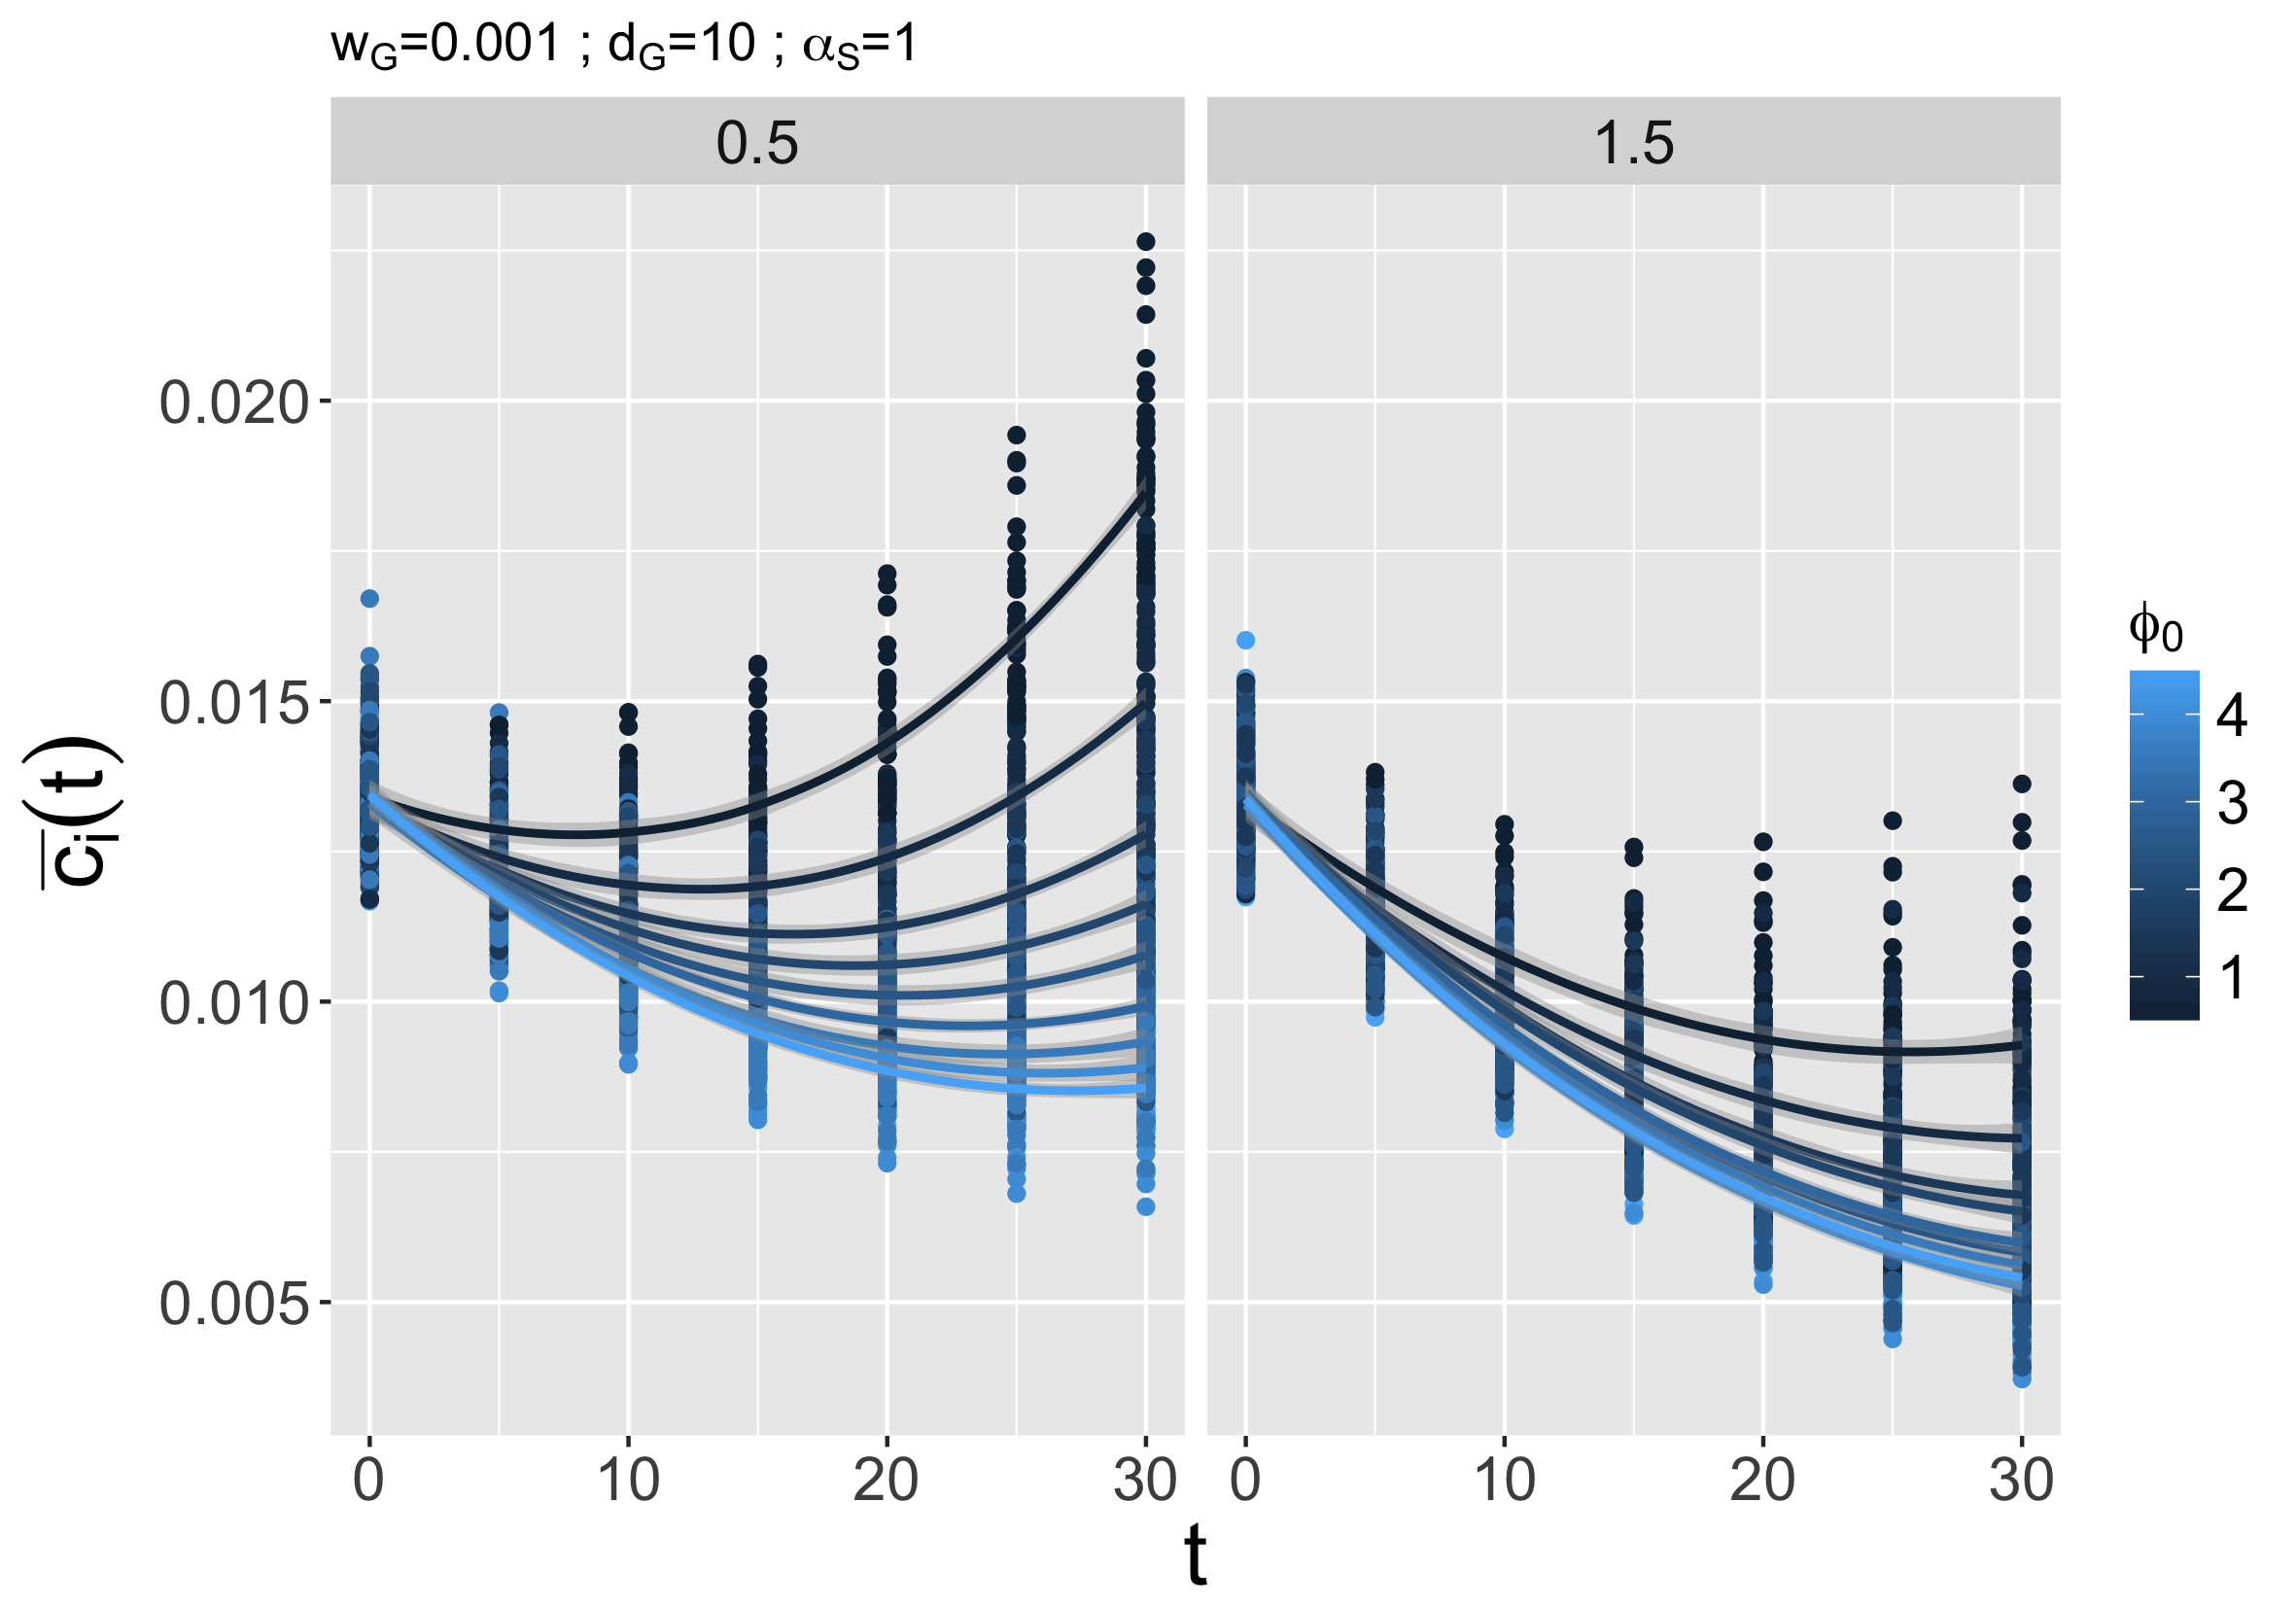
\includegraphics[width=0.48\linewidth]{Figures/MacroCoEvol/closenessSummaries_mean_synthRankSize1_gravityWeight0_001_gravityDecay10.png}\\
%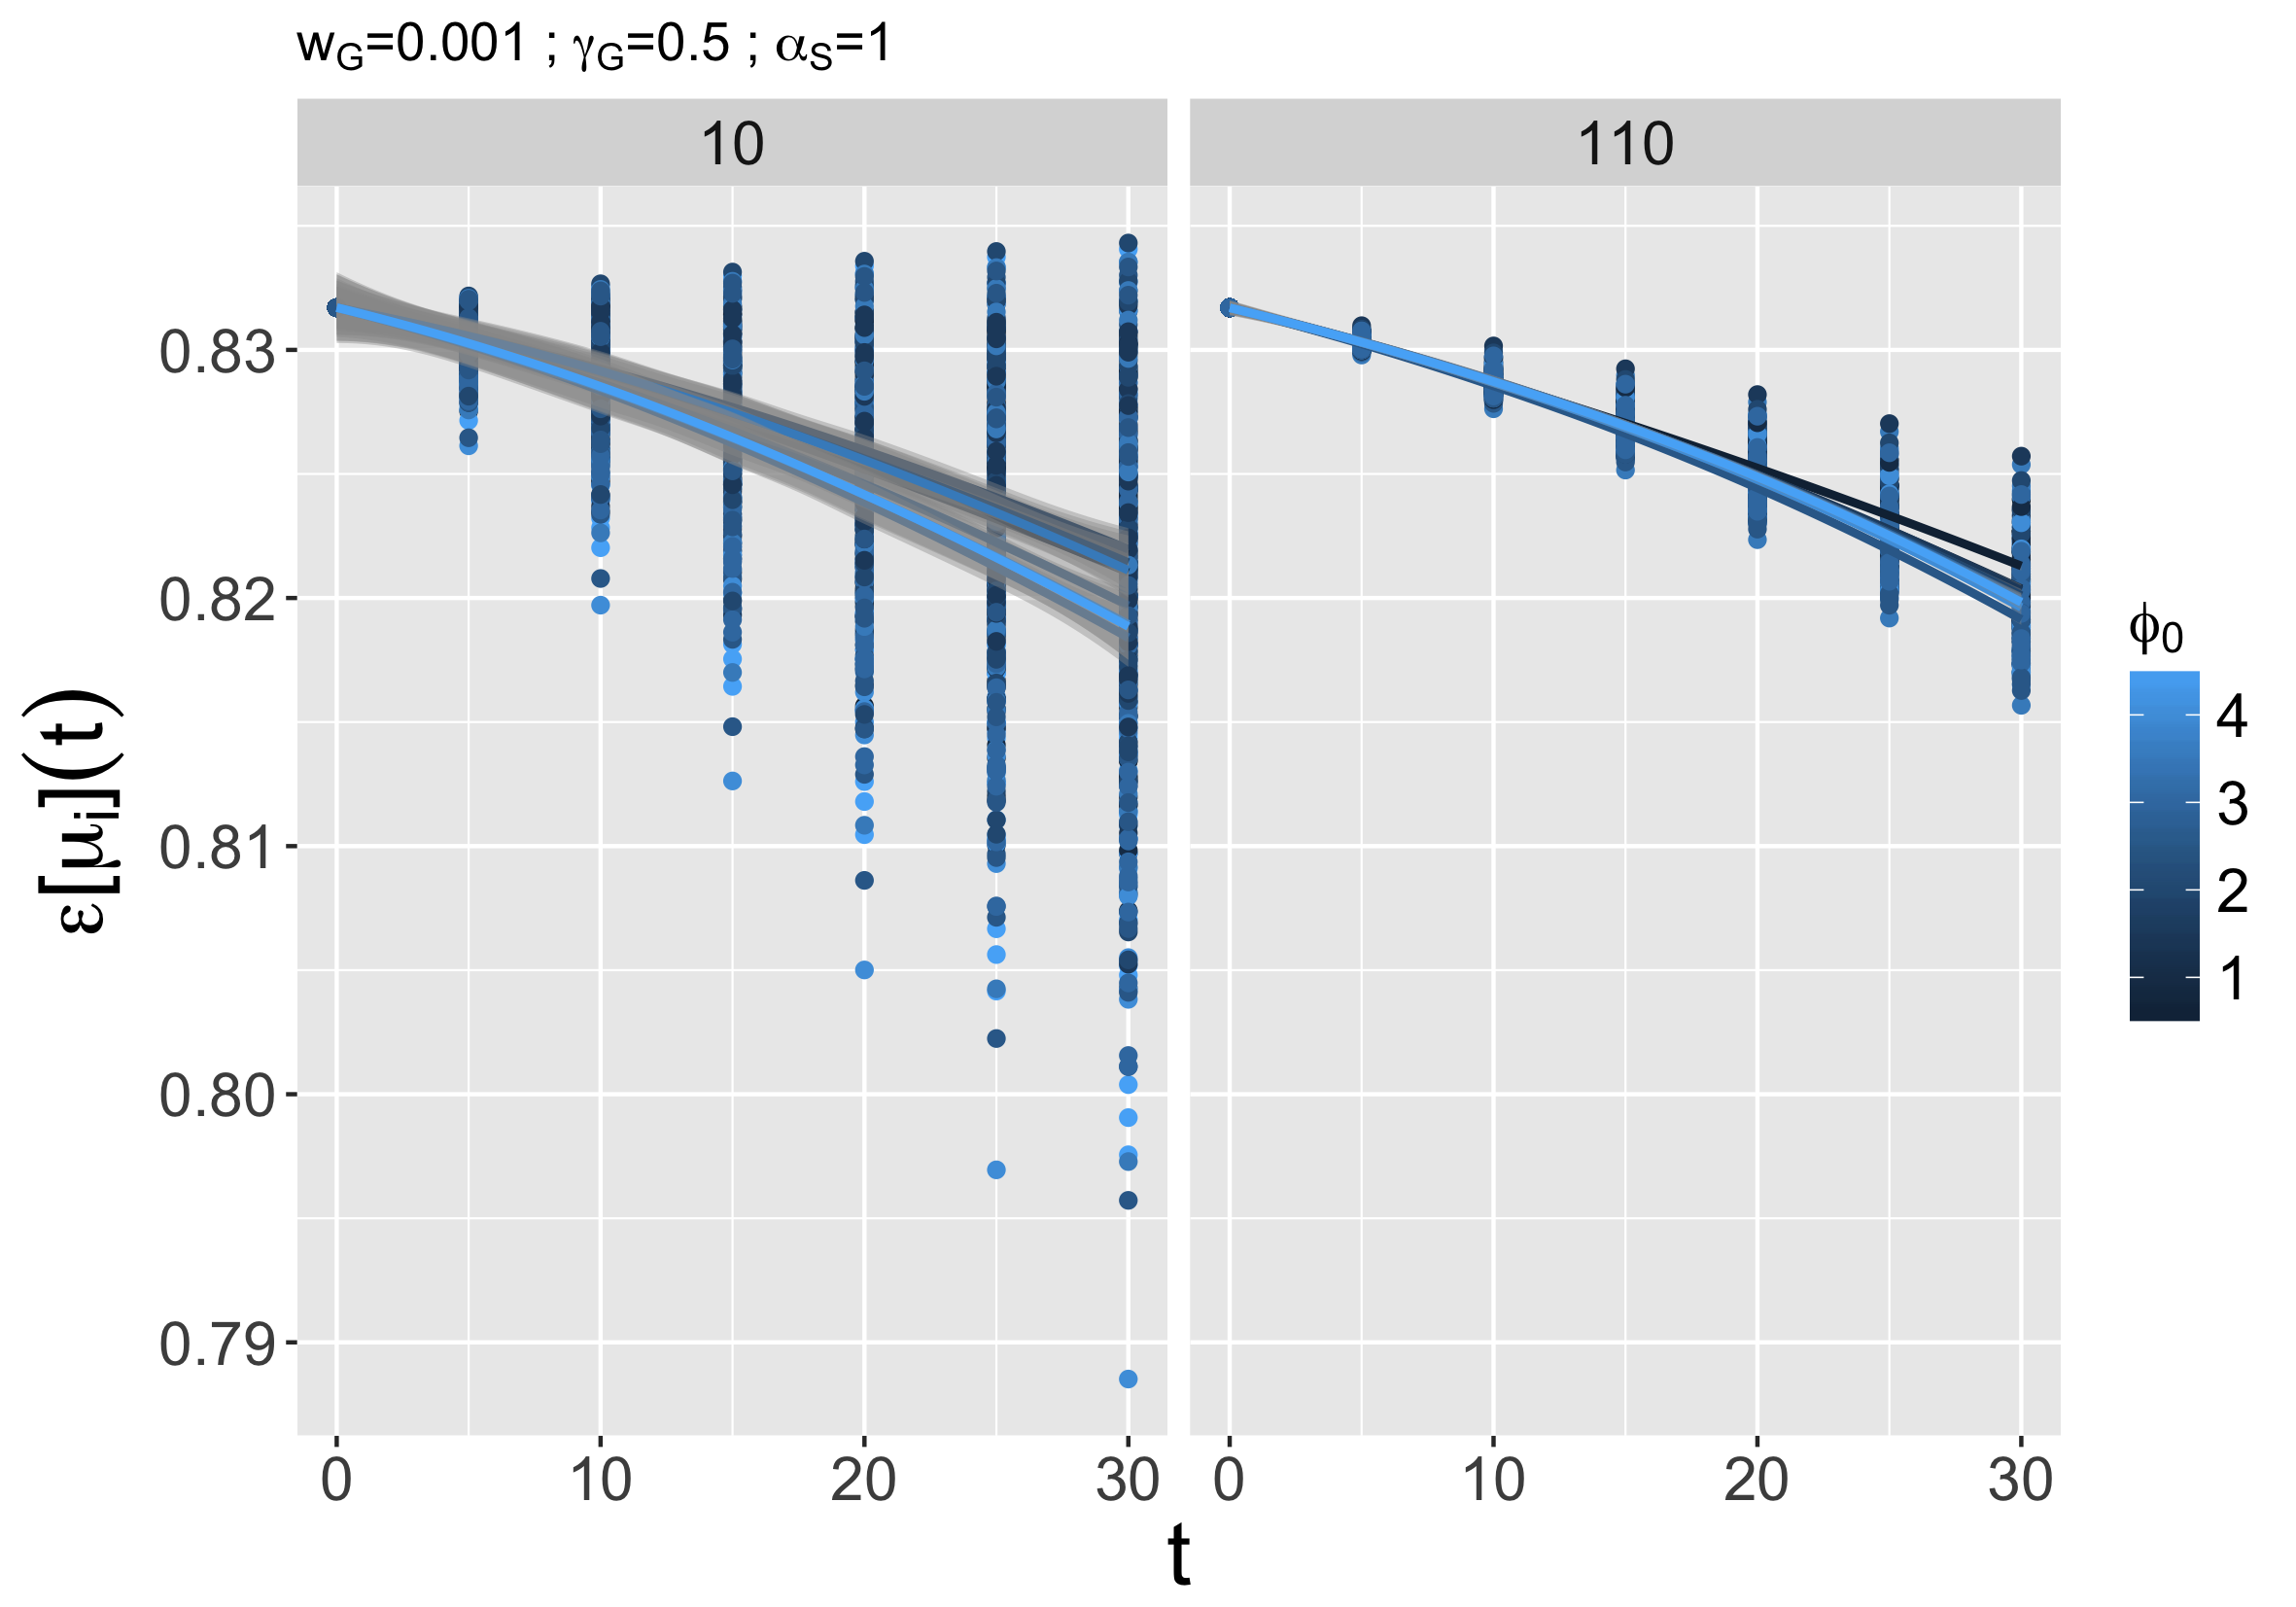
\includegraphics[width=0.48\linewidth]{Figures/MacroCoEvol/populationEntropies_synthRankSize1_gravityWeight0_001_gravityGamma0_5.png}
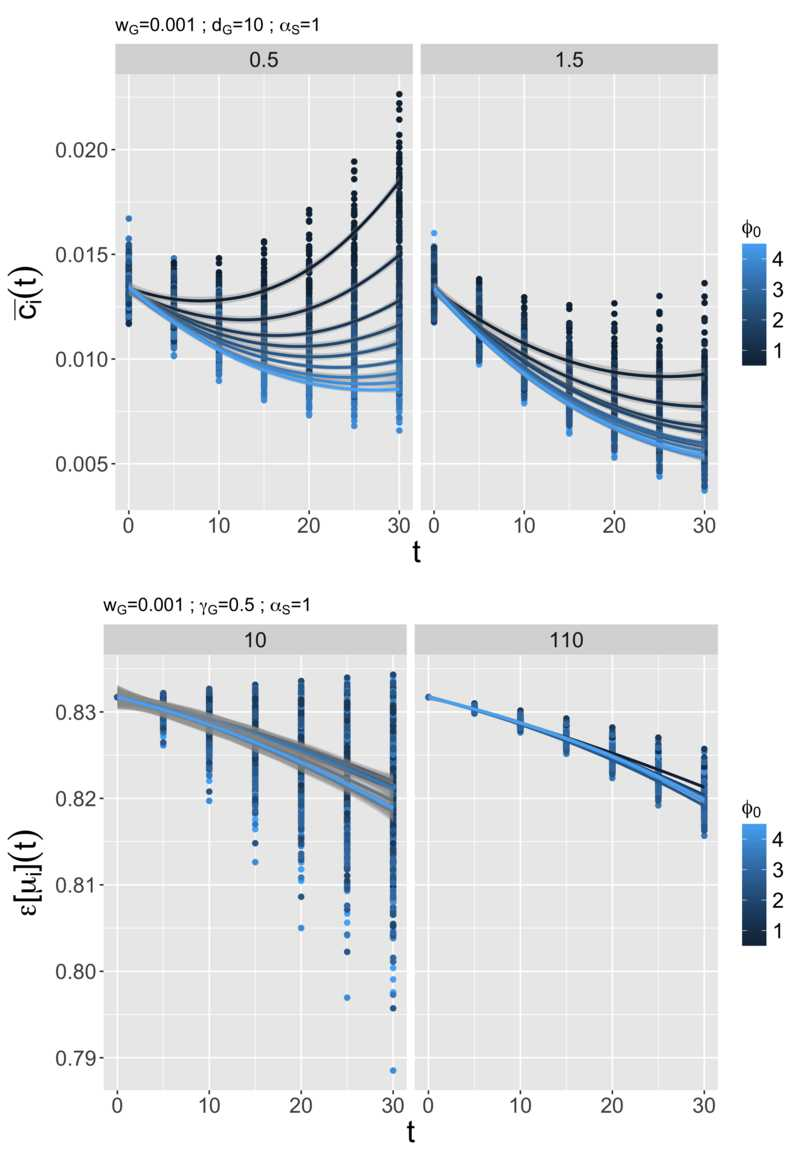
\includegraphics[width=\linewidth,height=0.9\textheight]{Figures/Final/6-2-2-fig-macrocoevol-behavior-time.jpg}
\caption[Behavior of the co-evolution model][Comportement temporel du modèle de co-évolution]{\textbf{Behavior of the co-evolution model.}\label{fig:macrocoevol:behavior-time}}{\textbf{Comportement temporel du modèle de co-evolution avec réseau abstrait sur un système de villes synthétique.} \textit{(Haut)} Moyenne des centralités de proximité, en fonction du temps, pour $\gamma_G$ (lignes) et $\phi_0$(couleur) variables, à $w_G = 0.001$ et $d_G = 10$ fixés ; \textit{(Bas)} Entropie de populations, en fonction du temps, pour $d_G$ (colonnes) et $\phi_0$(couleur) variables, à $w_G = 0.001$ et $\gamma_G = 0.5$ fixés. Se référer au texte pour l'interprétation. Les trajectoires sur la partie explorée de l'espace des paramètres sont données en Fig.~\ref{fig:app:macrocoevol:behavior-time}, Annexe~\ref{app:sec:macrocoevol}.\label{fig:macrocoevol:behavior-time}}
\end{figure}
%%%%%%%%%%%%%



%%%%%%%%%%%%%
\begin{figure}
%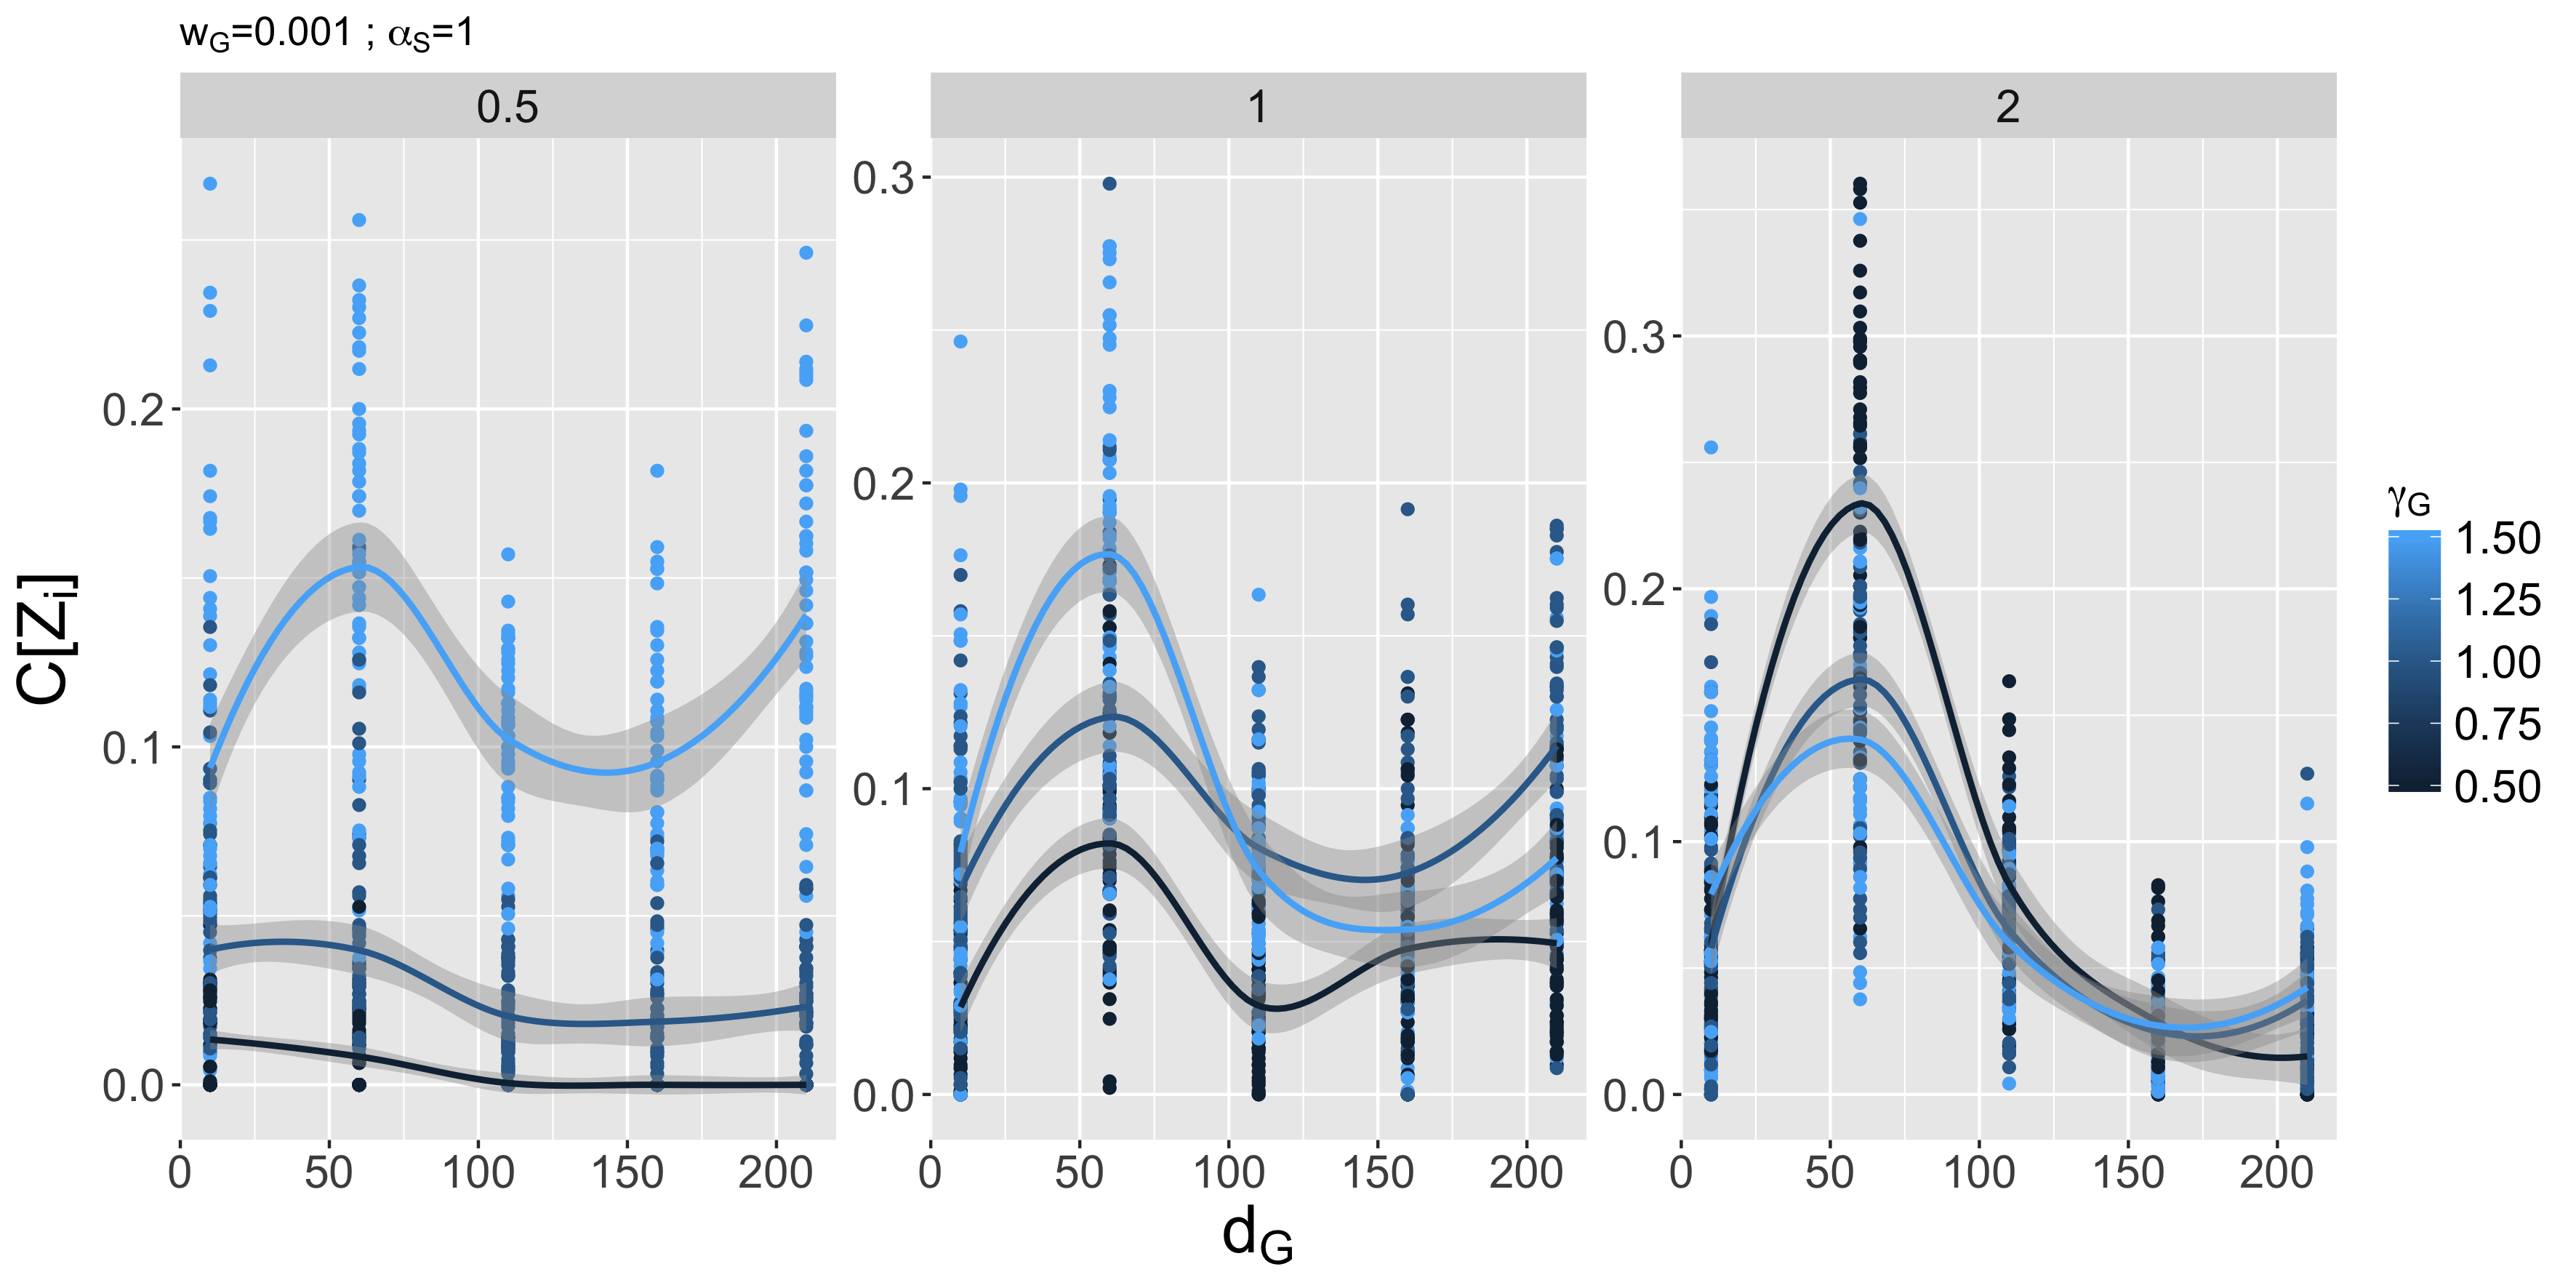
\includegraphics[width=0.48\linewidth]{Figures/MacroCoEvol/complexityAccessibility_synthrankSize1_nwGmax0_05_gravityWeight0_001.png}\\
% 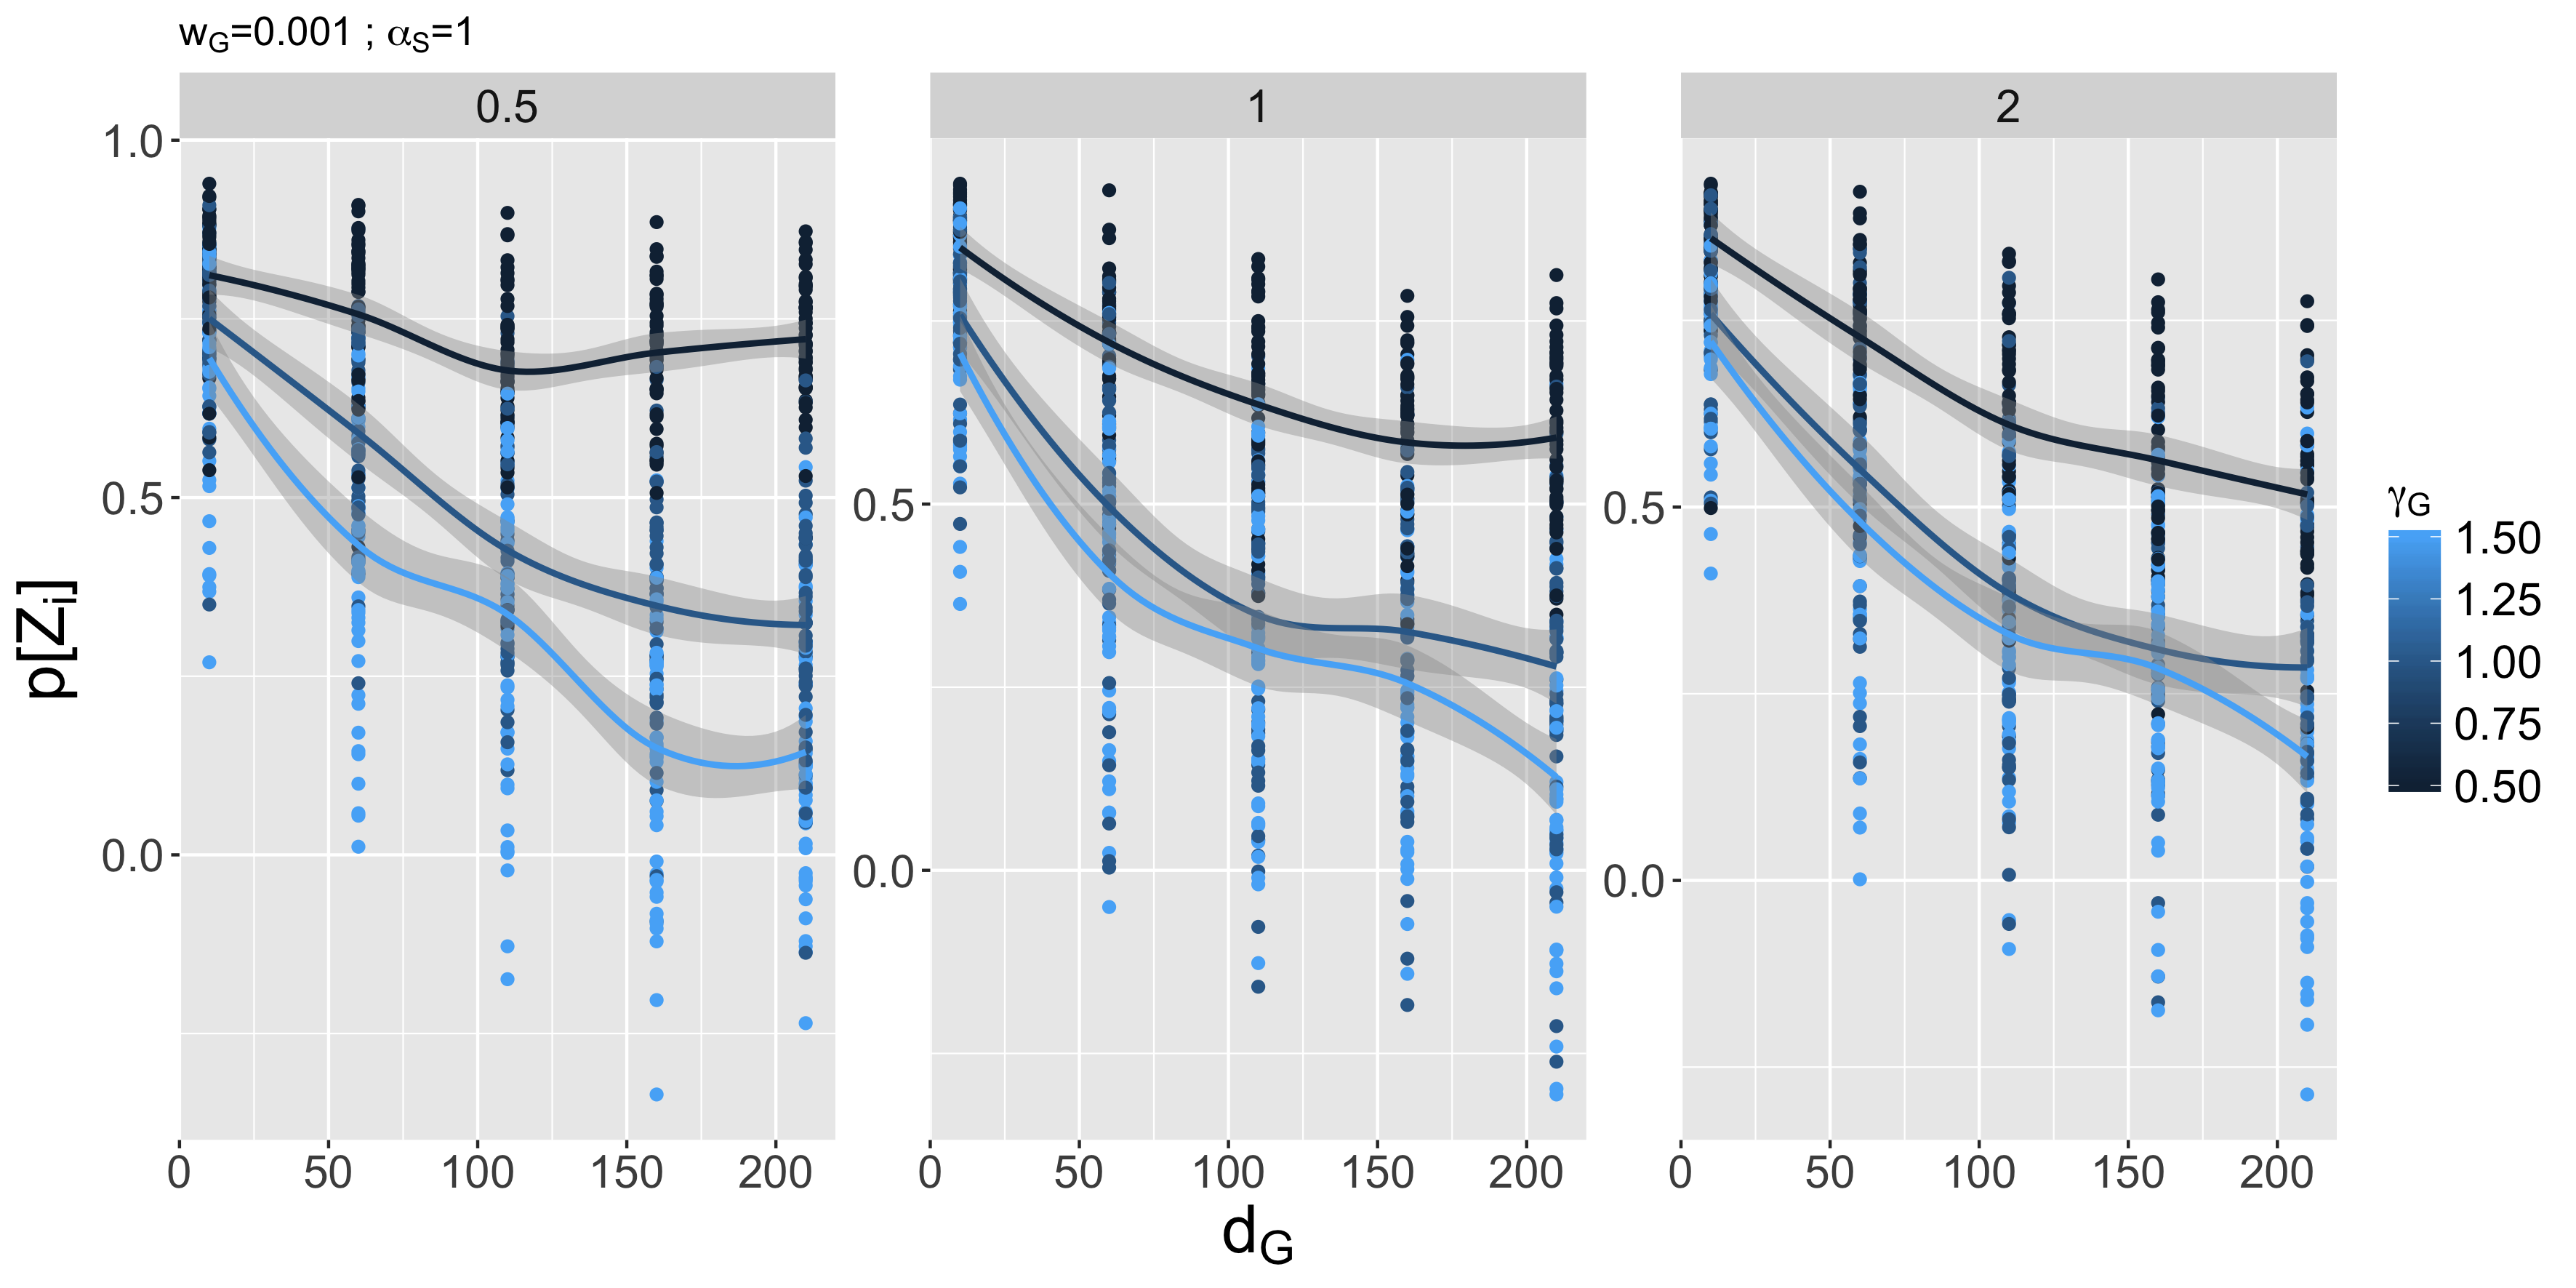
\includegraphics[width=0.48\linewidth]{Figures/MacroCoEvol/rankCorrAccessibility_synthrankSize1_nwGmax0_05_gravityWeight0_001.png}
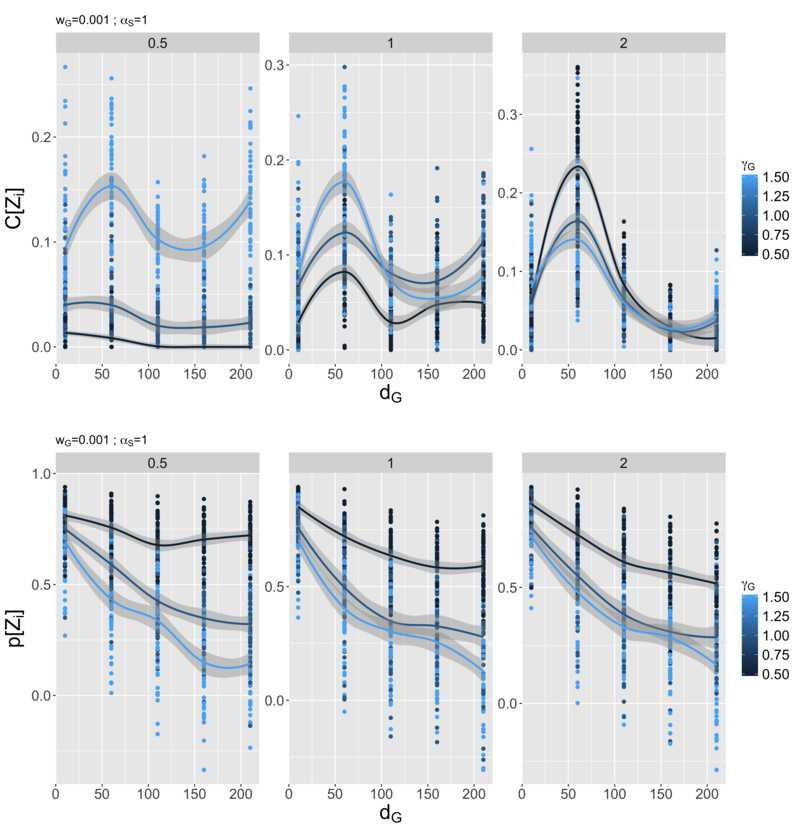
\includegraphics[width=\linewidth]{Figures/Final/6-2-2-fig-macrocoevol-behavior-aggreg.jpg}
\caption[Agregated behavior of the co-evolution model][Comportement agrégé du modèle de co-évolution]{}{\textbf{Comportement agrégé du modèle de co-evolution} \textit{(Haut)} Complexité des accessibilités, en fonction de $d_G$, pour $\phi_0$ (colonnes) et $\gamma_G$ (couleur) variables, à $w_G = 0.001$ fixé ; \textit{(Bas)} Corrélations de rang des accessibilités en fonction de $d_G$, pour les mêmes paramètres. Les comportements pour la partie explorée de l'espace des paramètres sont donnés en Fig.~\ref{fig:app:macrocoevol:behavior-aggreg}, Annexe~\ref{app:sec:macrocoevol}.\label{fig:macrocoevol:behavior-aggreg}}
\end{figure}
%%%%%%%%%%%%%



\subsubsection{Correlations}{Corrélations}



Nous pouvons dans un premier temps nous intéresser aux variations des corrélations entre variables en fonction de la distance. Les profils de $\rho_d$ pour les trois couples de variables montrent que des valeurs moyennes et grandes de la distance d'interaction ($d_G > 50$) induisent des populations totalement décorrélées aux centralités et accessibilités (Fig.~\ref{fig:app:macrocoevol:distcorrs}, Annexe~\ref{app:sec:macrocoevol}). Pour des petits $d_G$, un profil décroissant puis nul confirme l'existence d'effets locaux forts, où des villes très proches s'influenceront fortement. Le comportement de la corrélation entre accessibilité et centralité est plus difficile à interpréter, et peut être dû aux phénomènes d'auto-corrélation\footnote{Celles-ci ne sont pas calculables, car il s'agirait de décomposer $\rho\left[\sum_{i\neq j} \frac{1}{d_{ij}}; \sum_{i\neq j} P_j \exp{\left(-d_{ij}/d_G\right)}\right]$. Il est possible par exemple d'approximer $\rho\left[X+Y;Z\right]$ sous la condition que $\varepsilon = \sigma_Y / \sigma_X \ll 1$ au premier ordre par $\rho\left[ X+Y;Z \right] \simeq \left(\rho\left[ X;Z \right]  + \varepsilon \rho\left[Y;Z\right]\right)\cdot\left(1 - \frac{1}{2}\rho\left[X;Y\right]\varepsilon - \frac{\varepsilon^2}{2})\right)$, mais cette hypothèse est trop restrictive pour être valable sur l'ensemble de la somme.}. Son niveau ne dépend pas de la distance mais de $d_G$, et est décroissant pour finir à une corrélation négative.




\subsubsection{Causality regimes}{Régimes de causalité}


Tournons nous finalement vers les motifs de corrélations retardées produits par le modèle, c'est-à-dire l'étude de sa capacité à effectivement produire de la co-évolution comme nous l'avons définie.

L'exploration de profils de $\rho_{\tau}$ selon les paramètres est illustrée en Annexe~\ref{app:sec:macrocoevol}, et suggère l'existence de régimes de causalité variés. La Fig.~\ref{fig:macrocoevol:correlations} donne des exemples de profils. Nous constatons cependant (i) l'existence systématique d'une corrélation constante à $\tau = 0$ et (ii) les faibles variations des corrélations qui nécessitent la mise en place d'un test statistique pour être certains d'isoler un effet significatif.


Nous ajoutons donc ici un critère basé sur un test statistique : pour $\tau_+ = \textrm{argmax}_{\tau>0} \left|\rho_{\tau} - \rho_0\right|$ et $\tau_- = \textrm{argmax}_{\tau<0} \left|\rho_{\tau} - \rho_0\right|$, un test de Kolmogorov-Smirnov est utilisé pour comparer les distributions de $\rho_{\tau_{\pm}}$ et de $\rho_0$. S'il les déclare différentes avec une \emph{p-value} inférieure à $0.01$, et si $\left|\rho_{\tau_{\pm}}\right| > \left|\rho_0\right|$, nous convenons d'un lien de causalité entre les variables dans le sens correspondant.

Nous codons alors une configuration par une représentation de son graphe entre variables, donnée par les 6 variables discrètes valant 0 s'il n'y a pas de lien entre les variables (parmi l'ensemble des couples dirigés entre population, accessibilité et centralité) et 1 ou -1 selon le signe de la corrélation s'il existe un lien significatif statistiquement (en pratique toutes les corrélations sont positives).

Nous obtenons au total 33 configurations de liens entre variables, sur les 64 possibles ($2^6$ choix possibles pour des corrélations uniquement positives). En comparaison, l'application de cette méthode sur les résultats de~\ref{sec:macrocoevolexplo} ne donne que 8 configurations distinctes\footnote{Parmi lesquelles deux correspondent à une causalité circulaire négative entre accessibilité et centralité, ce qui fait dire que le modèle Simpopnet peut produire une co-évolution entre variables, mais en nombre restreint par rapport aux configurations obtenues ici et uniquement entre deux variables de réseau.}.

Les types de relations obtenues sont particulièrement éclairantes au regard de la co-évolution. On observe en effet :
\begin{itemize}
	\item une configuration sans lien entre variables ;
	\item 13 configurations de type ``effet structurant'', c'est-à-dire dont le graphe ne possède aucune boucle ; 
	\item une configuration de type ``co-évolution indirecte'', dont le graphe possède une boucle de longueur trois ($c_i \rightarrow X_i \rightarrow \mu_i \rightarrow c_i$)
	\item 18 configurations de type ``co-évolution'', dans lesquelles il existe au moins une boucle de longueur deux (relation circulaire directe entre deux variables).
\end{itemize}

%unique(signs$sign)
% [1] "01/00/00" "00/00/00" "11/00/00" "01/01/00" "11/00/10" "11/01/00" "11/01/10" "10/00/00" "10/00/10"
%[10] "10/10/10" "00/10/00" "00/01/00" "00/01/01" "00/00/11" "10/00/11" "00/11/00" "00/11/10" "10/01/10"
%[19] "00/01/11" "11/00/11" "01/00/10" "10/10/11" "00/11/11" "10/01/11" "00/01/10" "10/10/00" "10/11/00"
%[28] "10/11/10" "11/10/10" "00/10/11" "00/00/10" "10/11/11" "10/01/00"

%unique(signs$sign)[grep('11',unique(signs$sign))]
% [1] "11/00/00" "11/00/10" "11/01/00" "11/01/10" "00/00/11" "10/00/11" "00/11/00" "00/11/10" "00/01/11"
%[10] "11/00/11" "10/10/11" "00/11/11" "10/01/11" "10/11/00" "10/11/10" "11/10/10" "00/10/11" "10/11/11"

%unique(signs$sign)[grep('10/10',unique(signs$sign))]
%[1] "10/10/10" "10/10/11" "10/10/00" "11/10/10"

% unique(signs$sign)[grep('01/01',unique(signs$sign))]
% [1] "01/01/00" "00/01/01"

% unique(signs$sign[signs$strength>3])
%[1] "11/01/10" "11/00/11" "10/10/11" "00/11/11" "10/01/11" "10/11/10" "11/10/10" "10/11/11"


% SimpopNet
%  unique(signs$sign)
% [1] "00/00/00"   "00/00/-10"  "-1-1/00/00" "-10/00/00"  "00/00/10"   "-1-1/00/10" "00/10/00"   "0-1/00/00" 


Parmi tous ces régimes, 8 correspondent à un graphe avec au moins 4 liens (qui sont alors nécessairement co-évolutifs) : il s'agit des profils que nous représentons en Fig.~\ref{fig:macrocoevol:correlations}. Deux régimes présentent une déviation positive de la corrélation entre population et accessibilité pour les retards positifs, en croissance jusqu'au retard maximal, ce qui pourrait être un marqueur du renforcement des dynamiques de population par la centralité, fait stylisé exhibé pour le système de ville Français par~\cite{bretagnolle:tel-00459720}.

Les régimes où la centralité est en co-évolution avec la population correspondent à ceux où la co-évolution entre réseau et territoire est la plus marquée (puisque l'accessibilité relève des deux), et sont observés pour des grandes valeurs de $d_G$ (moyenne $d_G=183$ sur 62 points de paramètres). Ainsi, cette co-évolution est favorisée par de grandes portées d'interaction.

Enfin, le régime avec le plus fort nombre de liens\footnote{Correspondant au régime codé ``10/11/11'', avec co-évolution de la population et de la centralité ainsi que de la population et de l'accessibilité, et une causalité de la centralité sur l'accessibilité.}, est obtenu pour une grande portée d'interaction $d_G = 160$, une forte hiérarchie d'interaction $\gamma_G = 1.5$, mais une faible hiérarchie du système de ville initial $\alpha_S$ : des interactions lointaines et hiérarchisées dans un système uniforme conduisent à un maximum d'intrication entre variables.


%%%%%%%%%%%%%
\begin{figure}
	%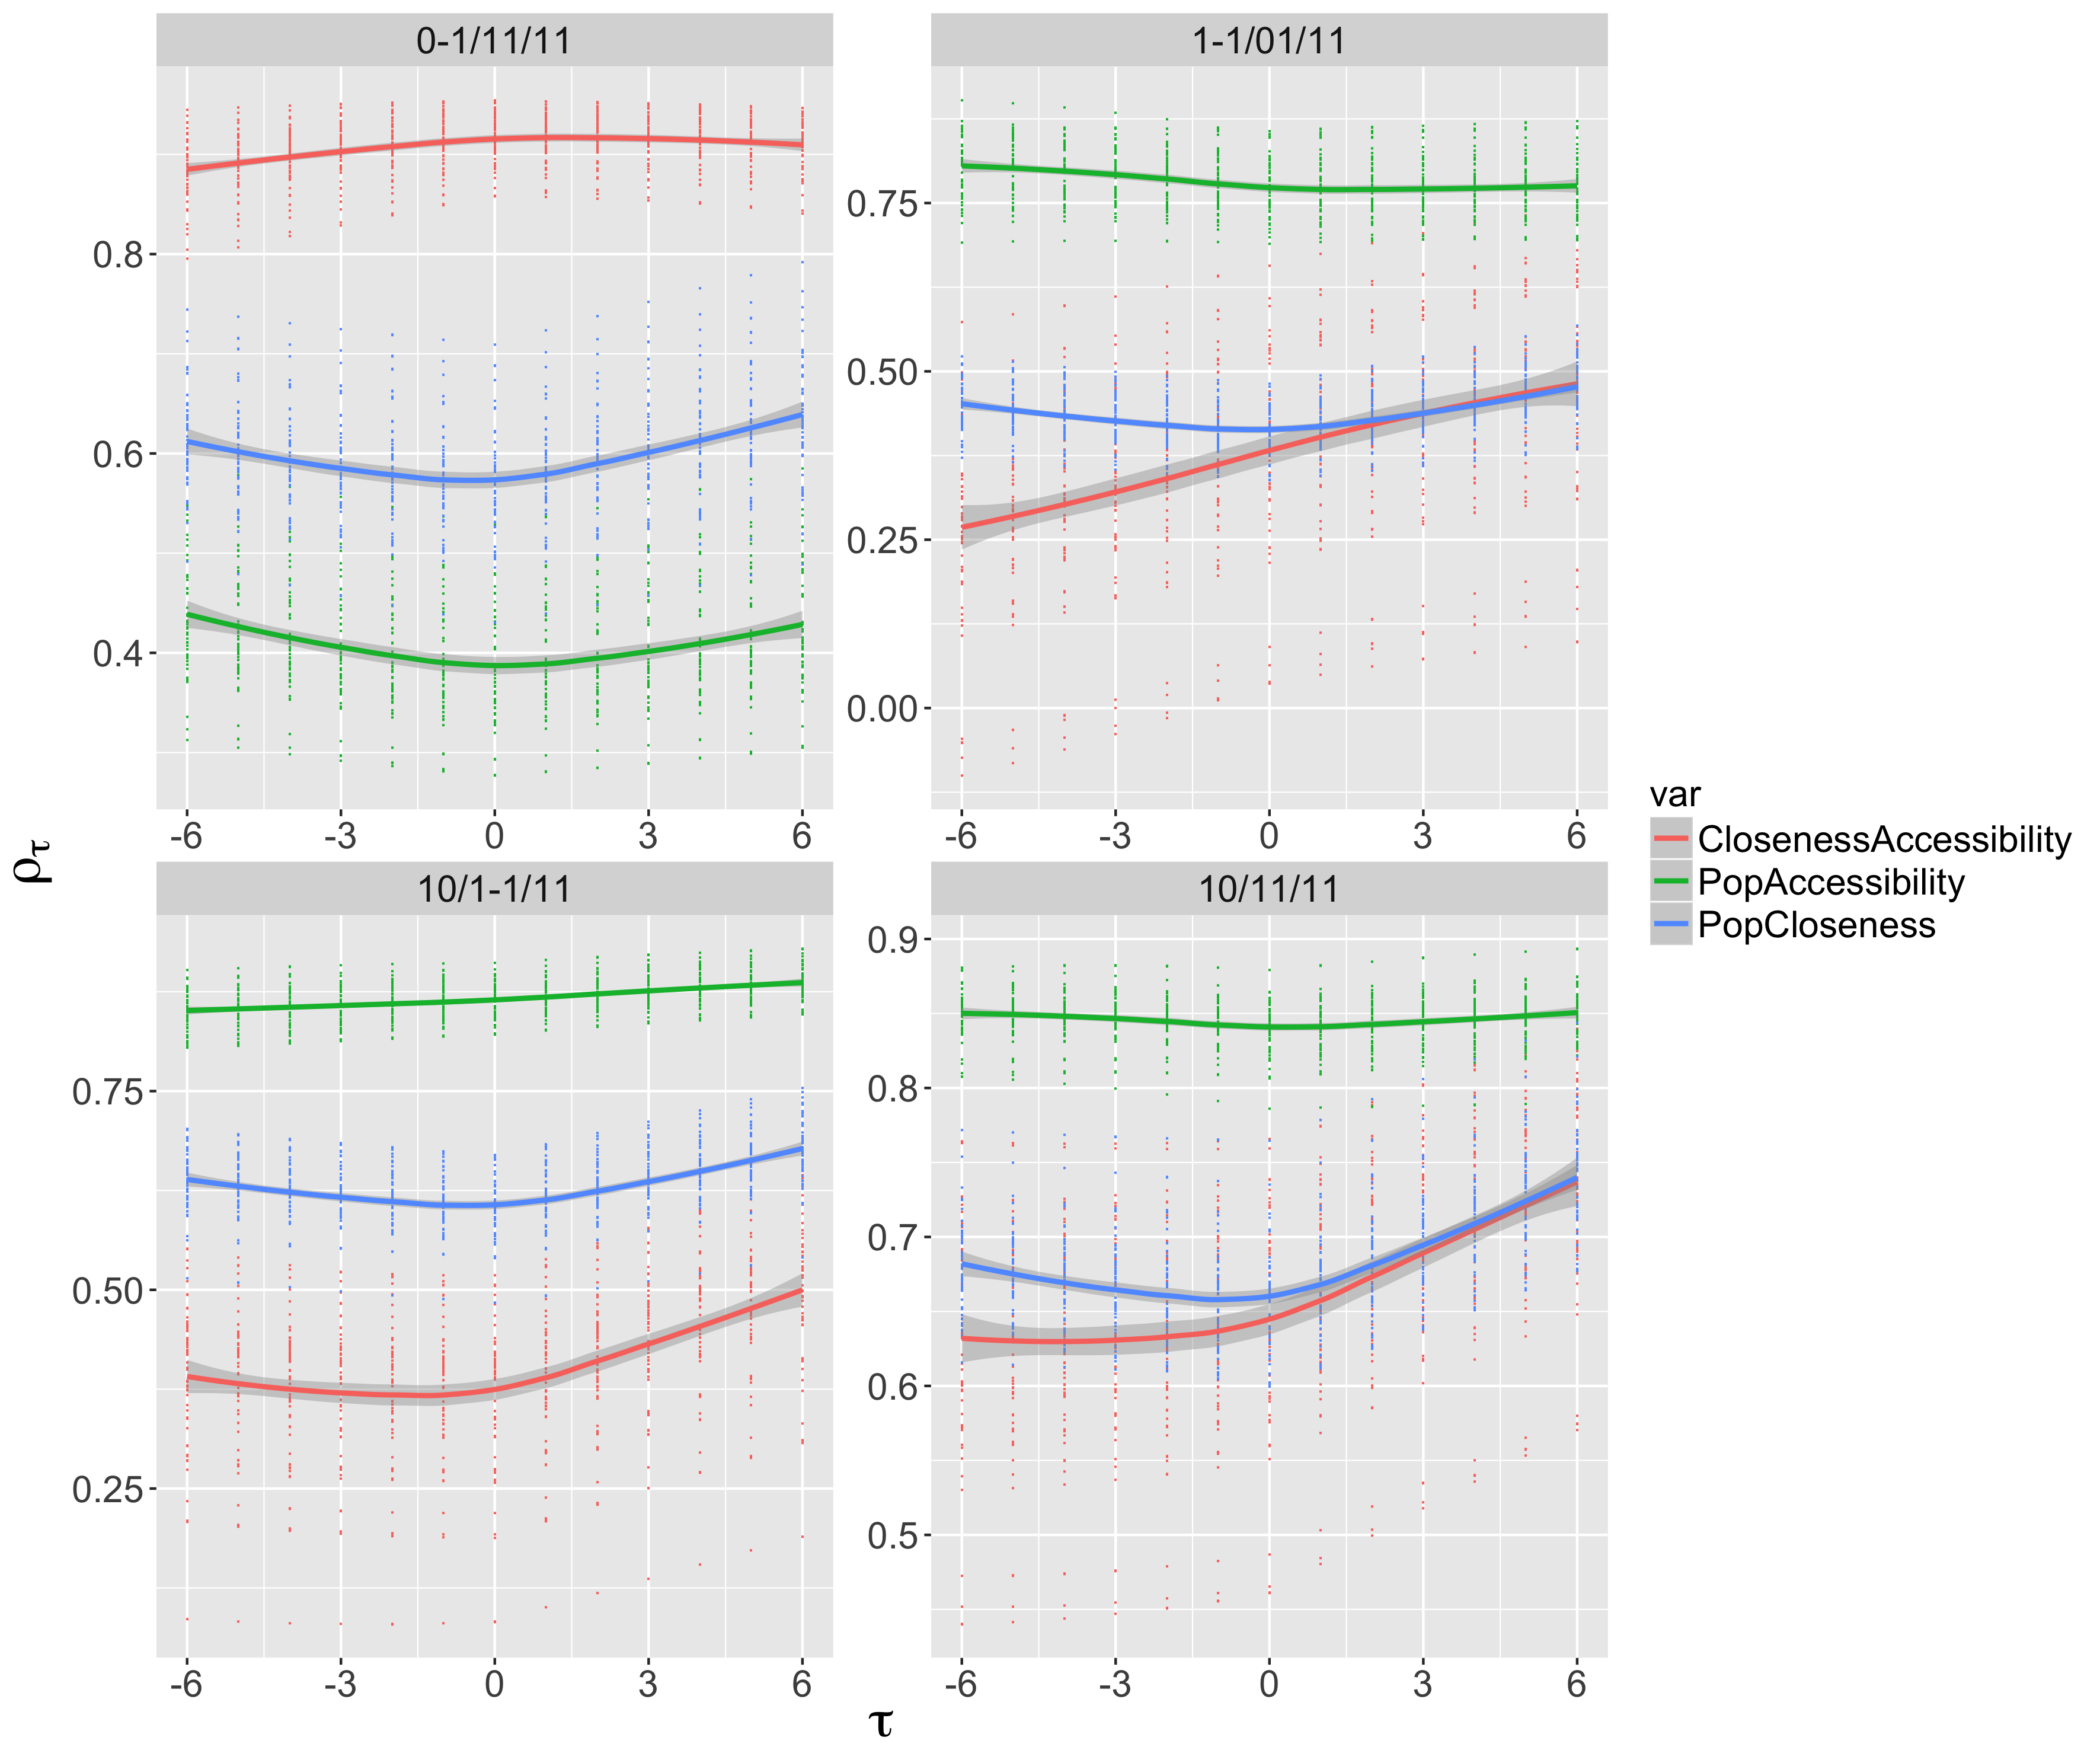
\includegraphics[width=\linewidth]{Figures/MacroCoEvol/laggedregimes_nwGmax0_05.png}
	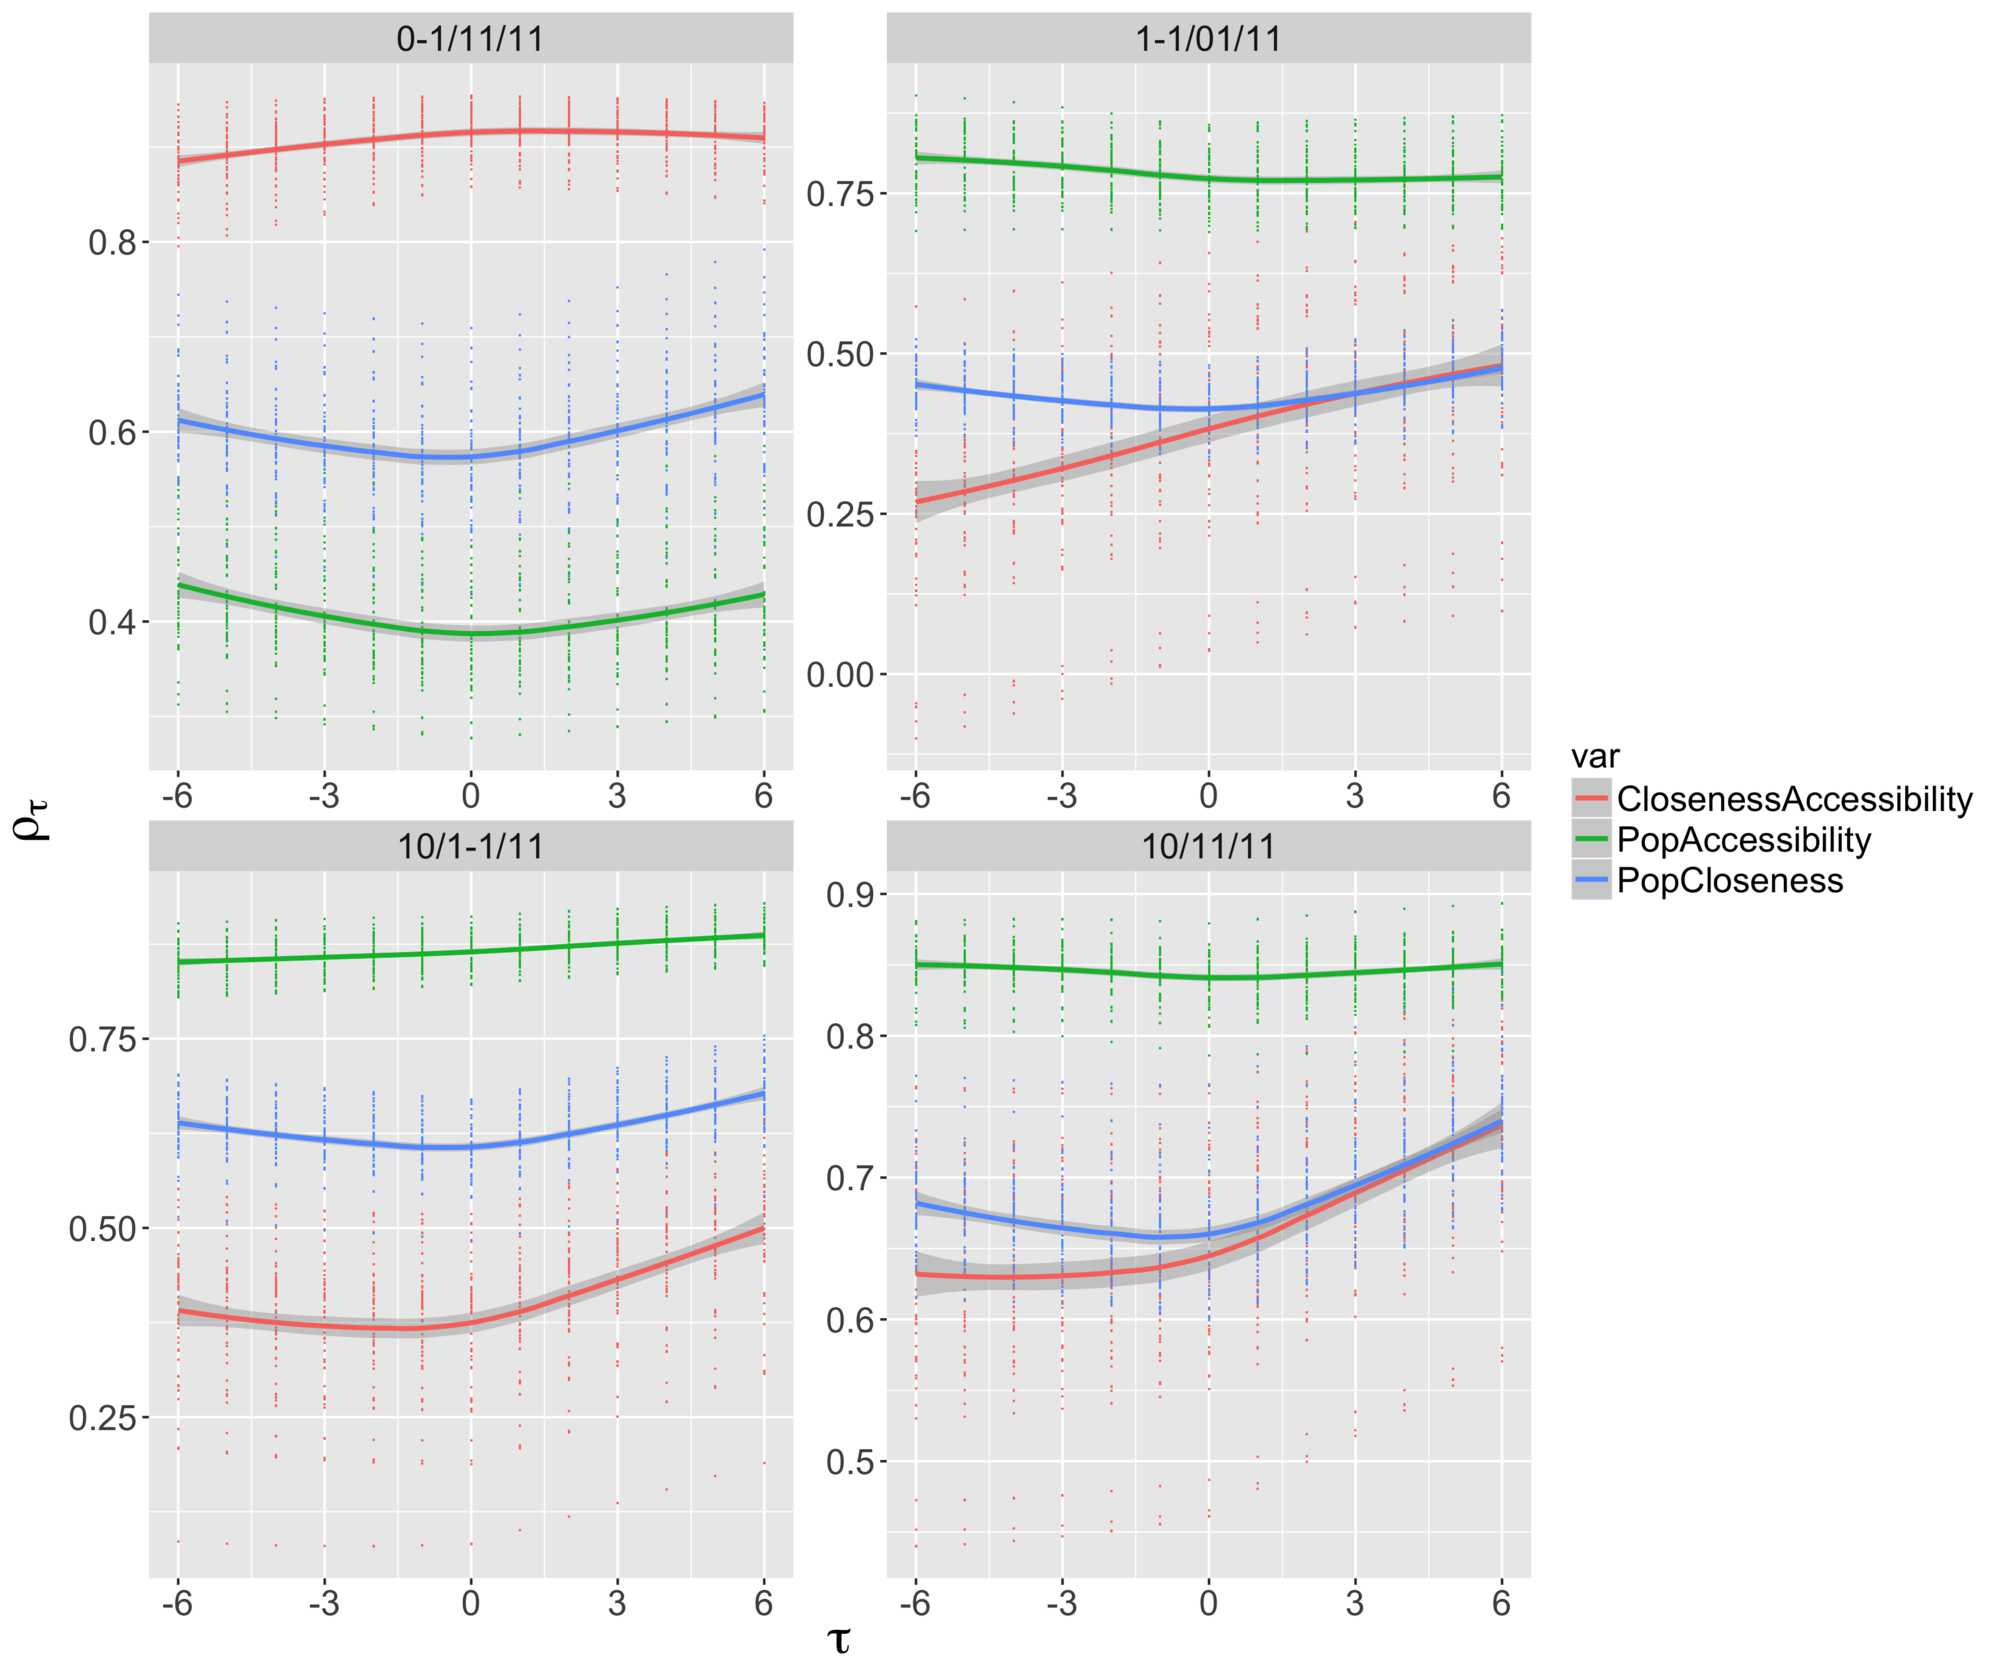
\includegraphics[width=\linewidth]{Figures/Final/6-2-2-fig-macrocoevol-correlations.jpg}
\caption[Correlations in the abstract model][Profils de corrélations retardées]{\textbf{Lagged correlations.} \label{fig:macrocoevol:correlations}}{\textbf{Corrélations retardées.} Nous donnons ici pour les 8 configurations présentant au moins 4 liens entre variables (codées dans l'ordre des couples, par l'existence ou non d'un lien pour $\tau_+$ puis pour $\tau_-$), les profils des corrélations retardées $\rho_{\tau}$ en fonction de $\tau$, pour l'ensemble des couples de variables (couleur).\label{fig:macrocoevol:correlations}}
\end{figure}
%%%%%%%%%%%%%


%summary(signs[signs$sign=="11/00/11"|signs$sign=="10/10/11"|signs$sign=="00/11/11"|signs$sign=="10/01/11"|signs$sign=="10/11/11",])
% synthRankSize        nwGmax     gravityWeight        nwThreshold     gravityGamma    gravityDecay  
% Min.   :0.5000   Min.   :0.05   Min.   :0.0002500   Min.   :2.500   Min.   :0.500   Min.   : 60.0  
% 1st Qu.:0.5000   1st Qu.:0.05   1st Qu.:0.0002500   1st Qu.:3.500   1st Qu.:1.000   1st Qu.:160.0  
% Median :0.5000   Median :0.05   Median :0.0005000   Median :4.000   Median :1.000   Median :210.0  
% Mean   :0.7419   Mean   :0.05   Mean   :0.0005444   Mean   :3.984   Mean   :1.105   Mean   :183.4  
% 3rd Qu.:1.0000   3rd Qu.:0.05   3rd Qu.:0.0007500   3rd Qu.:4.500   3rd Qu.:1.500   3rd Qu.:210.0  
% Max.   :1.5000   Max.   :0.05   Max.   :0.0010000   Max.   :4.500   Max.   :1.500   Max.   :210.0  
%     sign              strength      corrstrength   
% Length:62          Min.   :4.000   Min.   :0.1621  
% Class :character   1st Qu.:4.000   1st Qu.:0.2193  
% Mode  :character   Median :4.000   Median :0.2415  
%                    Mean   :4.016   Mean   :0.2397  
%                    3rd Qu.:4.000   3rd Qu.:0.2686  
%                    Max.   :5.000   Max.   :0.2914 


%signs[signs$sign=="10/11/11",]# max number of links
%  synthRankSize nwGmax gravityWeight nwThreshold gravityGamma gravityDecay     sign strength corrstrength
%1           0.5   0.05       0.00075         4.5          1.5          160 10/11/11        5    0.2274599


% plus resultats PSE

Nous confirmons finalement ces résultats de variété des régimes de causalité produits par le modèle en appliquant l'algorithme \emph{Pattern Space Exploration}~\cite{10.1371/journal.pone.0138212} au modèle, avec comme objectifs les 6 corrélations étudiées précédemment (évaluées comme nulles dans le cas d'une non-significativité). Une présentation graphique des résultats est donnée en Annexe~\ref{app:sec:macrocoevol}. Nous obtenons principalement un nombre de régimes produits par le modèle encore plus important que ceux obtenus précédemment (avec des corrélations négatives, 260 régimes réalisés sur $3^6 = 729$ possibles). Cette brève étude complémentaire confirme la capacité du modèle à produire une grande variété de régimes de co-évolution.




\subsubsection{Synthesis}{Synthèse}

Les faits stylisés marquants qui ressortent de l'exploration du modèle sur données synthétiques sont les suivants.

\begin{enumerate}
	\item On révèle l'existence d'une échelle spatiale intermédiaire permettant l'évolution de niches relativement indépendantes, correspondant à un niveau de complexité des trajectoires maximal.
	\item Les corrélations retardées mettent en évidence au moins trois régimes différents d'interaction, que l'on interprète comme un régime d'adaptation, un régime de co-évolution direct et un régime de co-évolution indirecte.
\end{enumerate}




%%%%%%%%%%%%%%%%%
%\subsection[Application][Application]{Applications to Case Studies}{Applications au Système de Villes Français}
\subsection{Applications to French City System}{Applications au système de villes français}



\bpar{
The model is applied to the French Urban System on long time dynamical data : Pumain-INED database for populations spanning between 1831 and 1999, with the evolving railway network from 1840 to 2000.
}{
Le modèle est ensuite appliqué au système de villes français sur des données dynamiques sur le temps long : la base Pumain-INED pour les populations, couvrant de 1831 à 1999~\cite{pumain1986fichier}, avec le réseau ferré dynamique de 1840 à 2000~\cite{thevenin2013mapping}. Cette durée temporelle découle de la logique des effets de structure sur le temps long, comme développé en~\ref{sec:networkterritories}. Cette application vise d'une part à tester la capacité du modèle à reproduire une dynamique de co-évolution réelle, et d'autre part à extraire une information thématique sur les processus via les valeurs calibrées des paramètres.
}



\subsubsection{Network Data}{Données de réseau}

Nous travaillons sur les données de réseau ferré construites par~\cite{thevenin2013mapping}. Le réseau ferré français est particulièrement intéressant en conjonction avec les données de population déjà présentées, puisque la période couverte est relativement similaire, et que comme le rappelle \cite{thevenin2013mapping}, ce moyen de transport a à toute période concrétisé l'implication d'acteurs publiques et privés importants, tout en correspondant à différents processus selon les époques, d'une gestion plutôt décentralisée à une centralisation très forte plus récemment, et différentes concrétisations technologiques avec par exemple l'émergence récente de la grande vitesse~\cite{zembri1997fondements}. Pour chaque date de la base de donnée de population, nous extrayons le graphe abstrait simplifié où toutes les gares et intersections de degré supérieur à deux sont reliés par les liens abstrait avec attributs de vitesse et distance traduisant la valeur réelle, à une granularité de 1km\footnote{Ce traitement est effectué grâce au package R pour l'analyse des réseaux de transport développé spécifiquement dans le cadre de cette thèse, voir~\ref{app:sec:packages}.}. Cela permet également de construire les matrices de distance-temps entre les villes considérées dans le modèle.




\subsubsection{Stylized facts}{Faits stylisés}


Avant de calibrer le modèle, observons les motifs de corrélation présents dans les données, en appliquant la méthode des corrélations retardées. Cette étude empirique devrait permettre d'une part de vérifier des faits stylisés connus, d'autre part d'établir une connaissance préliminaire du comportement empirique du système. Nous calculons comme précisé ci-dessus la centralité de proximité via le réseau, donnée par $T_i = \sum_j \exp{-d_{ij}/d_0}$, et étudions la corrélation retardée entre sa dérivée $\Delta T_i$ et celle de la population $\Delta P_i$, donnée par $\hat{\rho}_{\tau} = \hat{\rho}\left[\Delta P_i(t),\Delta T_i(t-\tau)\right]$ estimée sur une fenêtre glissante comprenant $T_w$ dates successives. Nous montrons en Fig.~\ref{fig:macrocoevol:empirical} les résultats obtenus.


Ces résultats sont importants pour au moins deux raisons. Dans un premier temps, le comportement du nombre de corrélations significatives en fonction de $T_w$ et de $d_0$ permet la recherche d'échelles de stationnarité dans le système. Nous observons d'une part une échelle spatiale spécifique donnant un maximum pour l'ensemble des fenêtres temporelles, à $d_0 = 100km$, ce qui suggère l'existence de sous-systèmes régionaux cohérents, dont l'existence est stable dans le temps : en effet, cette valeur correspond à la distance d'interaction . Celle-ci coincide remarquablement avec l'échelle intermédiaire isolée dans le modèle synthétique. D'autre part, les grandes portées spatiales induisent une échelle temporelle optimale, pour $T_w = 4$ ce qui correspond à une vingtaine d'année : nous l'identifions comme l'échelle de stationnarité temporelle du système dans son ensemble et étudions les corrélations retardées pour cette valeur.


Dans un second temps, le comportement des corrélations retardées ne semble pas en accord avec la littérature existante. À l'échelle spatiale intermédiaire, les valeurs de $\rho_+,\rho_-$ n'exhibent aucune régularité. Sur l'ensemble du système, on a jusqu'en 1946 quasiment aucun effet significatif, puis aucune causalité entre 1946 et 1975 (maximum à $\tau = 0$, minimum non significatif), puis un décalage de 5 ans de l'accessibilité causant la population après 1968 (l'effet restant tout de même douteux). Nous ne reproduisons pas l'effet de corrélation entre centralité dans le réseau et place dans la hiérarchie urbaine défendu par~\cite{bretagnolle2003vitesse}\footnote{Tout comme~\cite{lemoy2017scaling} n'arrivent pas à reproduire, pour les profils de densité en fonction de la distance au centre des métropoles européennes, la transition permettant à \cite{guerois2008built} de définir le péri-urbain. Ces travaux plus ou moins anciens ne sont pas reproductibles, ne fournissant ni code, ni données et ne donnant qu'une description très succincte des méthodes, et il est ainsi impossible de connaitre l'origine de la divergence qualitative obtenue. Une bonne reproductibilité ainsi que la construction de comparaisons systématiques (\emph{benchmarks}) de modèles, analyses empiriques, récentes mais aussi en validation d'études passées, nous semble une bonne solution à ce genre de problèmes.}, ce qui amène à relativiser l'existence de la ``co-évolution structurelle'' sur le temps long décrite par \noun{Bretagnolle} dans~\cite{espacegeo2014effets}. Ce que trouve \cite{bretagnolle2003vitesse}, c'est une correspondance simultanée entre taux de croissance et niveau de connectivité aux réseaux (et non avec les dynamiques du réseau), mais pas à notre sens une co-évolution, d'autant plus qu'aucune relation statistique n'est exhibée.


Nous rejoignons les résultats récents de~\cite{mimeur:hal-01616746} qui montrent le non-significativité statistique de la corrélation entre taux de croissance et évolution de la couverture du réseau ainsi que l'évolution de l'accessibilité, à délai nul. Nos résultats sont moins précis pour les classes de villes étudiées (ils différencient grandes villes et petites, et travaillent sur un panel plus grand), mais plus généraux car pour un délai et une portée de l'accessibilité variables, et donc complémentaires.



%%%%%%%%%%%%%
\begin{figure}
	%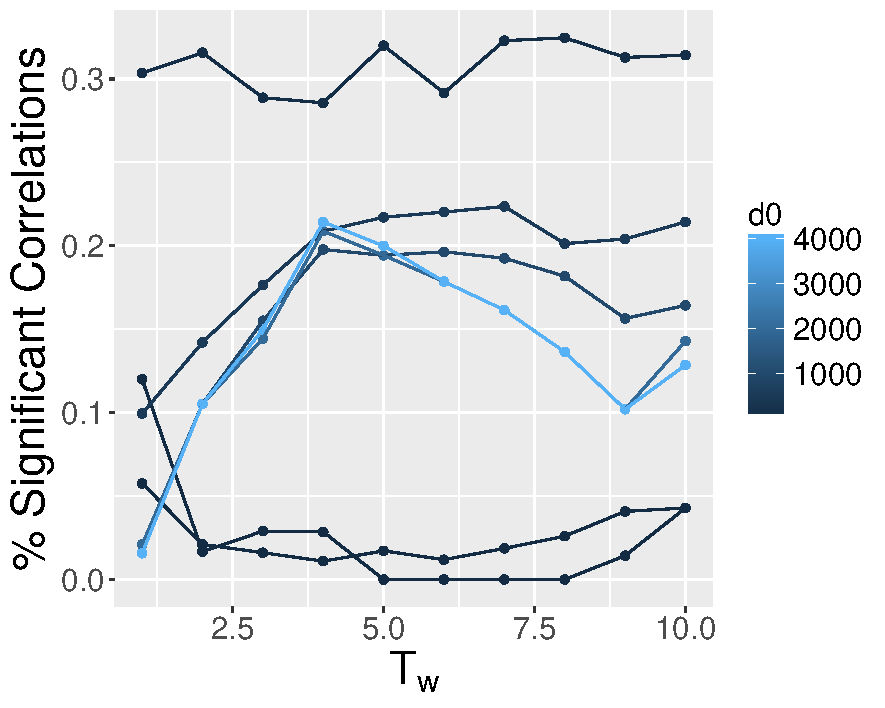
\includegraphics[width=0.48\linewidth]{Figures/MacroCoEvol/significantcorrs_Tw.pdf}
	%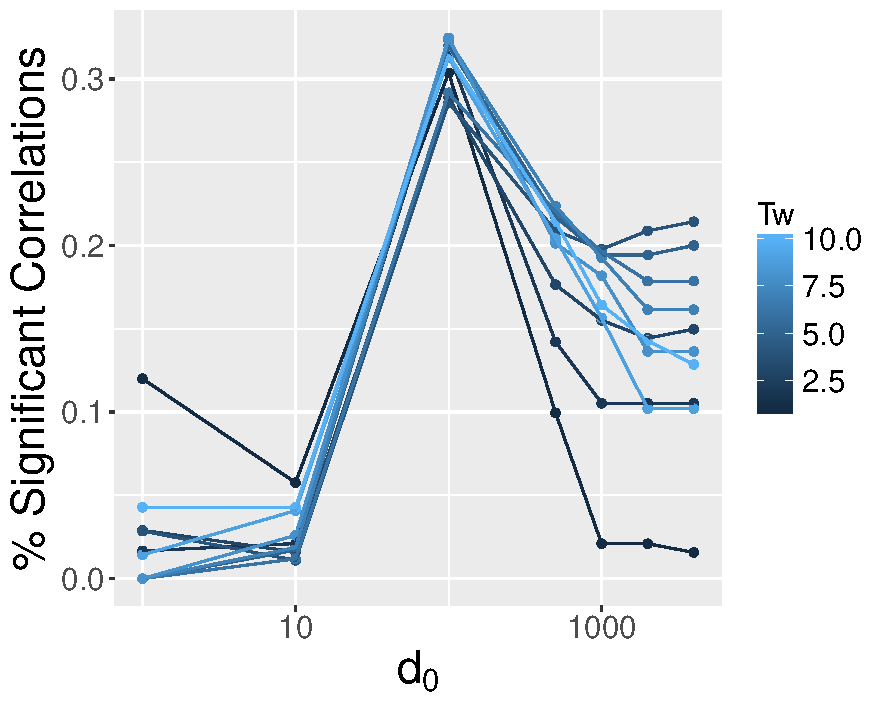
\includegraphics[width=0.48\linewidth]{Figures/MacroCoEvol/significantcorrs_d0.pdf}\\
	%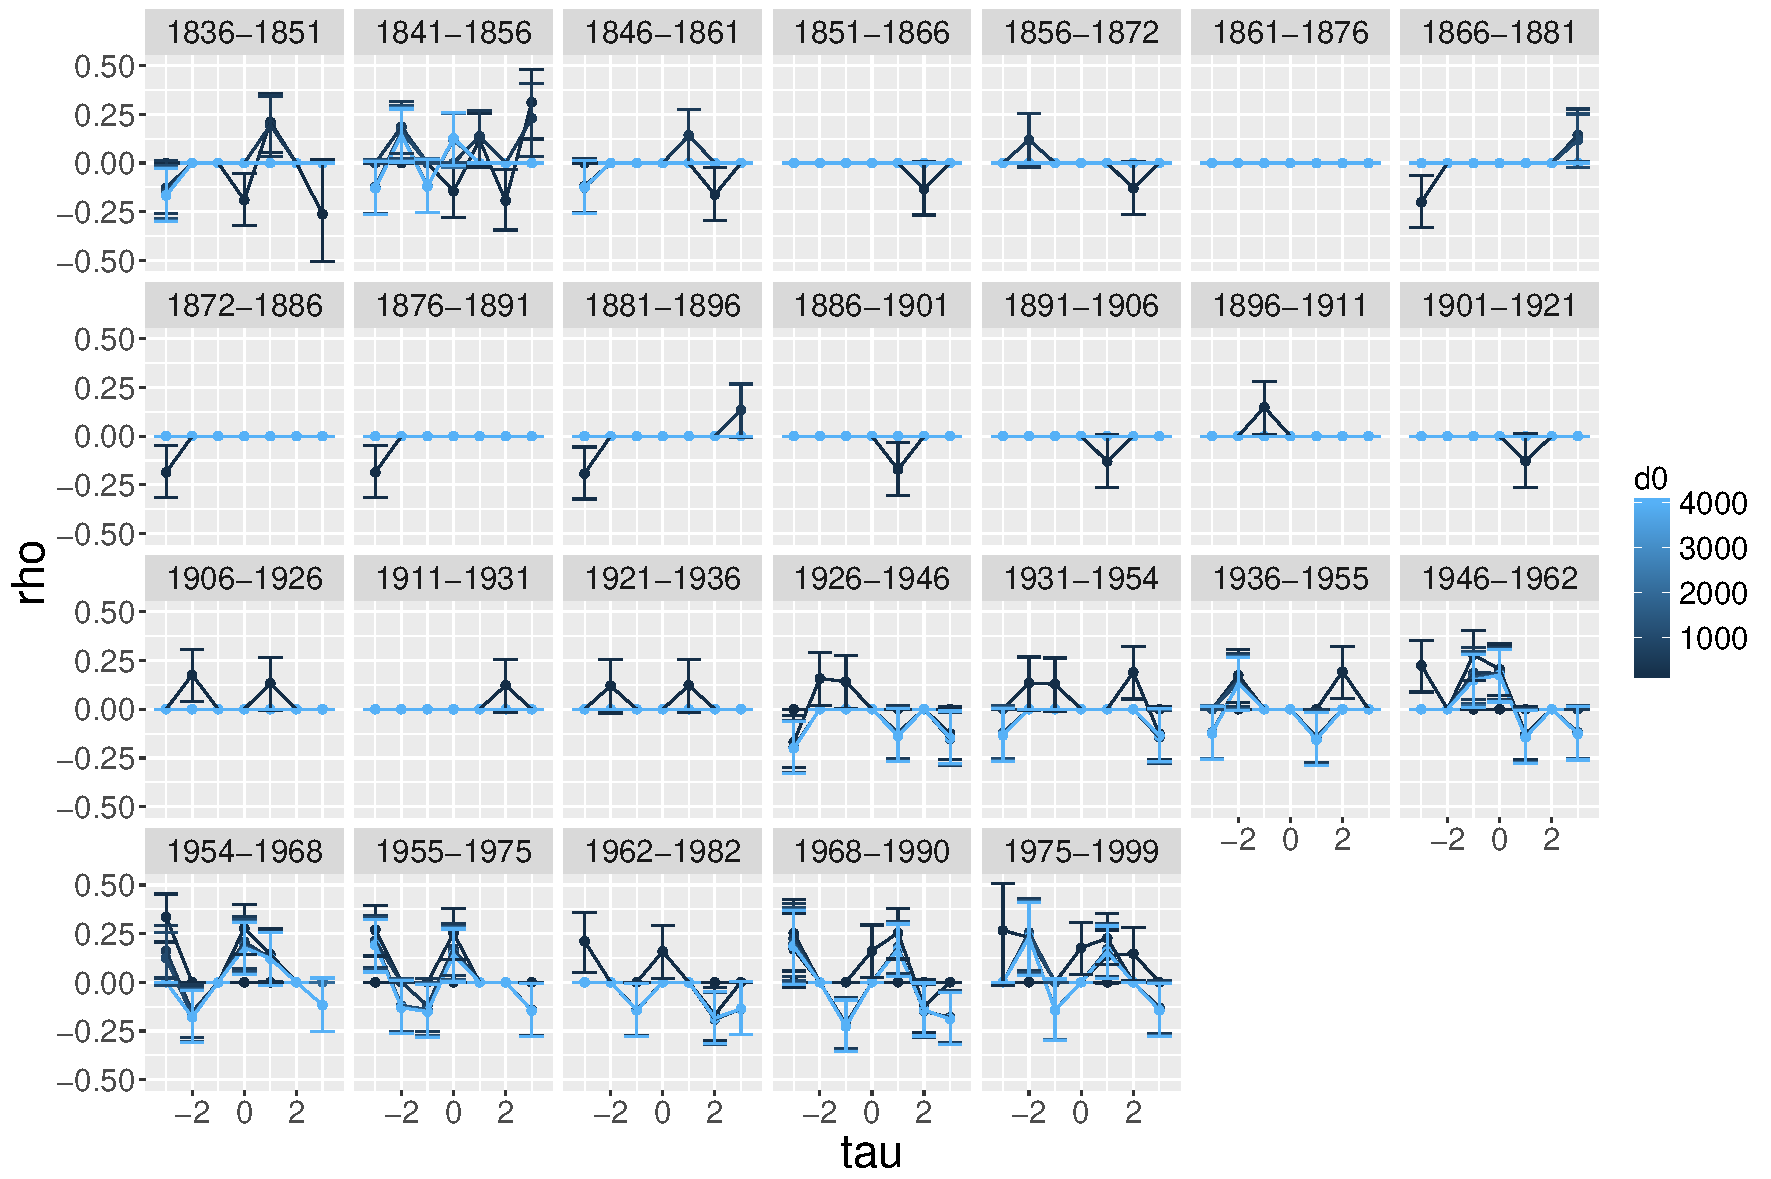
\includegraphics[width=\linewidth]{Figures/MacroCoEvol/laggedCorrs_time_Tw4.pdf}
	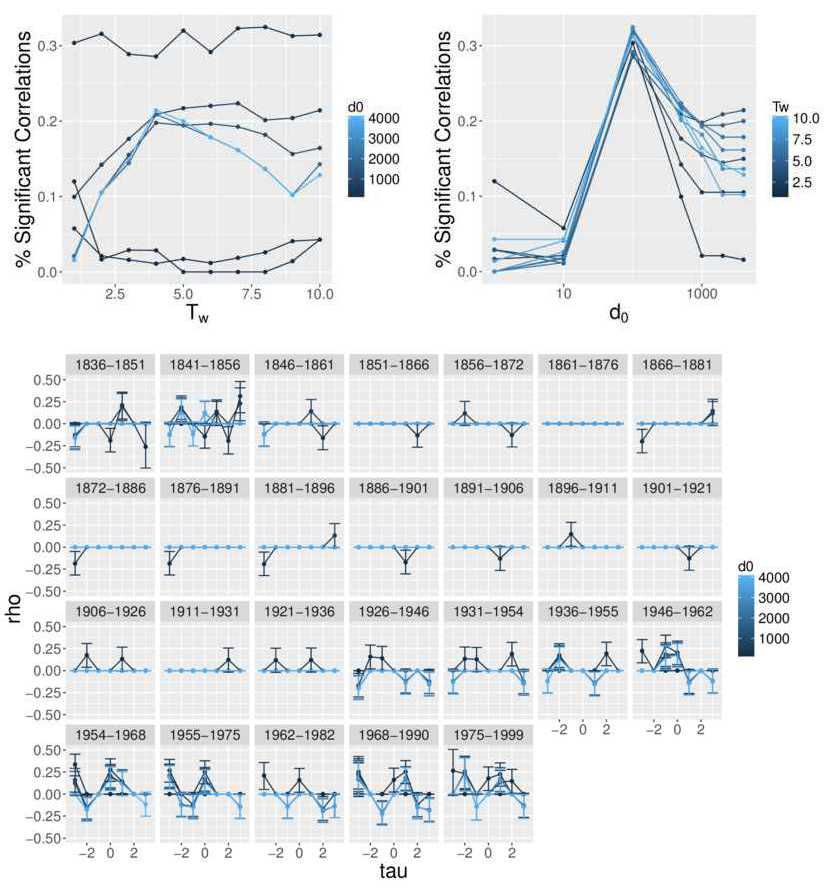
\includegraphics[width=\linewidth]{Figures/Final/6-2-3-fig-macrocoevol-empirical.jpg}
	\caption[Empirical Lagged Correlations for French City System][Corrélations empiriques pour le système de villes français]{\label{fig:macrocoevol:empirical}}{\textbf{Corrélations retardées empiriques pour le système de villes français.} Les corrélations sont calculées sur une fenêtre de taille $5\cdot T_w$, entre les taux de croissance des populations et ceux de centralité de proximité avec un paramètre de décroissance $d_0$ (voir texte). \textit{(Haut Gauche)} Nombre de corrélation significatives (prises telles que $p<0.1$ à 95\%) en fonction de $T_w$ pour $d_0$ variable ; \textit{(Haut droite)} Nombre de corrélations significatives en fonction de $d_0$ pour $T_w$ variable ; \textit{(Bas)} Pour la fenêtre ``optimale'' $T_w=4$, valeur de $\rho_{\tau}$ en fonction de $\tau$, pour l'ensemble des périodes successives.\label{fig:macrocoevol:empirical}}
\end{figure}
%%%%%%%%%%%%%









\subsubsection{Abstract model calibration}{Calibration du modèle abstrait}


\bpar{
Expected results concern both accurate city population growth reproduction, and network patterns, i.e. how does taking into account dynamical networks can introduce further exploratory power in such models for population trajectories, and also how realistic network distance evolution is.
}{
Les résultats attendus de la calibration sur données réelles concernent à la fois la reproduction plus ou moins précise des dynamiques réelles de croissance de population, c'est-à-dire dans quelle mesure la prise en compte d'un réseau dynamique peut augmenter le pouvoir explicatif pour les trajectoires, et aussi quel est le niveau de réalisme de l'évolution de la distance par le réseau. Nous travaillons toujours avec le modèle abstrait.
}


\paragraph{Model evaluation}{Evaluation du modèle}

On peut ajouter aux indicateurs utilisés précédemment un indicateur de calibration pour la distance. L'aspect particulier de l'ajustement pour les populations, qui résidait dans la présence d'une loi de puissance pour les tailles de villes rendant négligeables les performances sur les villes moyennes et les petites villes dans le cas d'une erreur cumulée, et suggérait l'ajout de l'indicateur de l'erreur sur les logarithmes, n'est pas présent pour les distances qui suivent une distribution concentrée sur un ordre de grandeur unique. Nous utilisons ainsi une mesure standard d'ajustement, donnée par
\[
\varepsilon_D = \log \left[ \sum_t \sum_{i,j} \left(d_{ij}(t) - \tilde{d}_{ij}(t)\right)^2\right]
\]
où $d_{ij}(t)$ sont les distances observées et $\tilde{d}_{ij}(t)$ les distances simulées. Il s'agit simplement d'une erreur carré cumulée, comme utilisée pour la comparaison de matrices origine-destination dans un cas similaire de simulation d'un réseau de transport dans~\cite{jacobs2016transport}.


%%%%%%%%%%%%%
%% ON HOLD : benchmark static model with real network distances


%\paragraph{Role of Real Network Distances}{Rôles des distances réelles de réseau}

%\bpar{
%We use as a benchmark network the geographical shortest paths that have been shown in a previous work to already capture network effects (see~\cite{raimbault2016models} and section~\ref{sec:interactiongibrat}).
%}{
%Nous utilisons comme réseau de benchmark les plus courts chemins géographiques qui ont été montrés déjà capturer des effets de réseaux dans un précédent travail (voir~\cite{raimbault2016models} et la section~\ref{sec:interactiongibrat}).
%}




\paragraph{Results}{Résultats}


Nous procédons à une calibration non-stationnaire, sur les objectifs $(\varepsilon_P,\varepsilon_D)$, c'est-à-dire l'erreur carrée sur les population et celle sur les distances. L'estimation est faite par fenêtre mobile sur les périodes déjà utilisées en~\ref{sec:interactiongibrat}. Pour limiter la dimension à explorer, nous fixons $w_N = 0$ pour n'étudier que les interactions au premier ordre, sachant que les paramètres de réseau abstrait $(g_{max},\gamma_S,\varphi_0)$ sont pris en compte dans la calibration. La calibration est effectuée par algorithme génétique de façon similaire à~\ref{sec:interactiongibrat}. La Fig.~\ref{fig:macrocoevol:pareto} montre les fronts de Pareto obtenus, et la Fig.~\ref{fig:macrocoevol:parameters} l'évolution dans le temps des valeurs des paramètres pour les solution optimales.


Nous observons une forte variabilité des formes des fronts de Pareto pour la calibration bi-objectif population et distance, ce qui témoigne d'une plus ou moins grande difficulté à ajuster simultanément population et distance. Certaines périodes, comme 1891-1911 et 1921-1936, sont proches de présenter un point optimal simultané pour les deux objectifs, ce qui correspondrait à une bonne adéquation du modèle à la fois aux trajectoires de villes et à celle du réseau sur ces périodes.

En comparaison aux résultats de calibration sur le modèle avec réseau statique de~\ref{sec:interactiongibrat}, en regardant les performances pour l'objectif $\varepsilon_G$, nous trouvons des périodes où le statique est clairement meilleur (1831 et 1841 par exemple) et d'autres où le modèle co-évolutif est meilleur (1946 et 1962) : ainsi, la prise en compte de la co-évolution permet dans certains cas une meilleure reproduction des trajectoires de population.


Les valeurs des paramètres optimaux dans le temps, présentées en Fig.~\ref{fig:macrocoevol:parameters}, contiennent un certain signal. L'évolution de $w_G$ et $\gamma_G$ sont consistantes avec celles observées pour le modèle statique. Pour $d_G$, le modèle sature principalement sur une distance maximale et l'évolution est difficile à interpréter. 

Par contre, l'évolution de $\phi_0$ pourrait témoigner d'un ``effet TGV'' dans les instants récents, par le pic secondaire pour la population après 1960. En effet, la construction des LGV a raccourci les distances entre les villes au plus haut de la hiérarchie, et une augmentation du seuil $\phi_0$ correspond à une augmentation de la sélectivité pour une diminution potentielle des distances.

Le $g_{max}$ calibré peut enfin être interprété selon l'histoire du réseau ferré (du moins pour l'ensemble des points du font de Pareto) : un pic significatif dans les premières années, un creux dans les années de stabilisation du réseau (1900), puis une augmentation jusqu'à aujourd'hui liée à l'augmentation de la vitesse des trains puis l'ouverture des lignes à grande vitesse.

Nous avons pu ainsi dans une certaine mesure indirectement quantifier les processus d'interaction par le réseau et ceux d'adaptation du réseau au flux, dans le cas d'un système réel.

%%%%%%%%%%%%%%%%%%%
\begin{figure}
%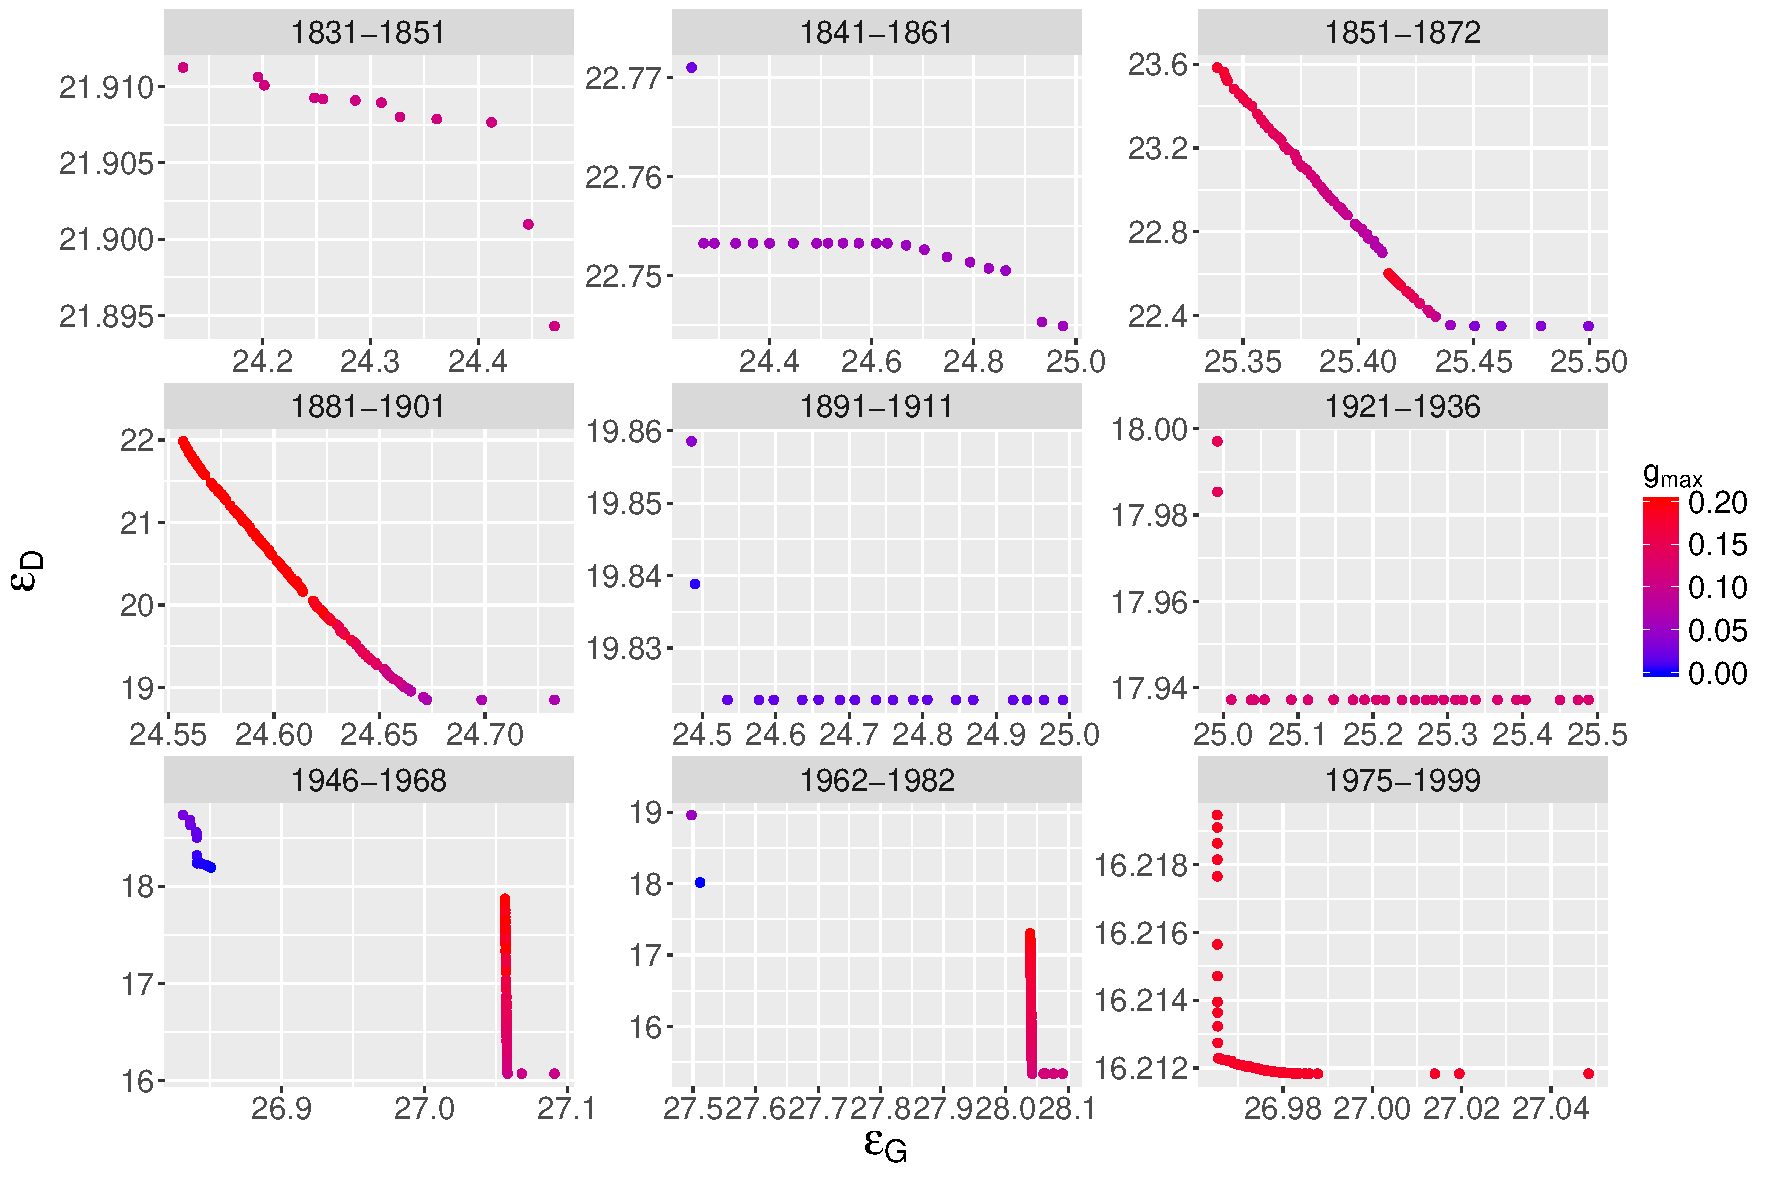
\includegraphics[width=0.9\linewidth]{Figures/MacroCoEvol/pareto_nwGmax_filtTRUE.pdf}
	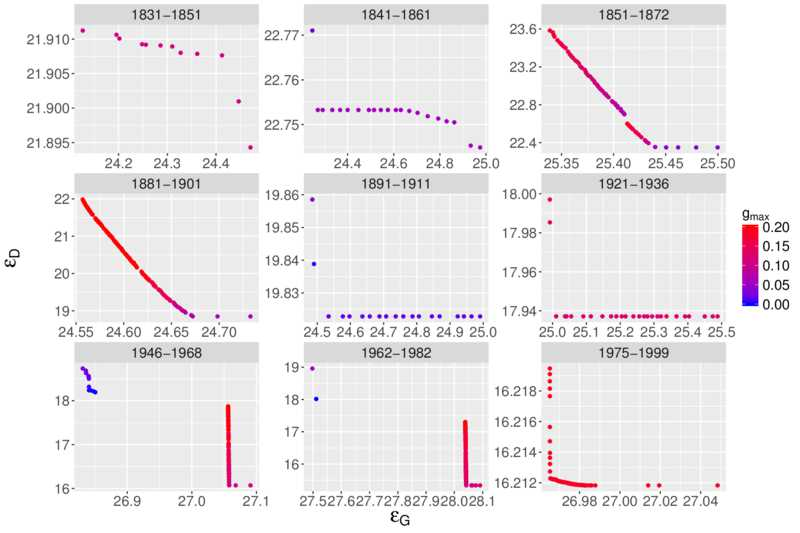
\includegraphics[width=\linewidth]{Figures/Final/6-2-3-fig-macrocoevol-pareto.jpg}
	\caption[Pareto fronts][Fronts de Pareto pour la calibration sur population et distance]{\label{fig:macrocoevol:pareto}}{\textbf{Fronts de Pareto pour la calibration bi-objectif population et distance.} Les fronts sont donnés pour chaque période de calibration, et colorés en fonction de $g_{max}$.\label{fig:macrocoevol:pareto}}
\end{figure}
%%%%%%%%%%%%%%%%%%%



%%%%%%%%%%%%%%%%%%%
\begin{figure}
	%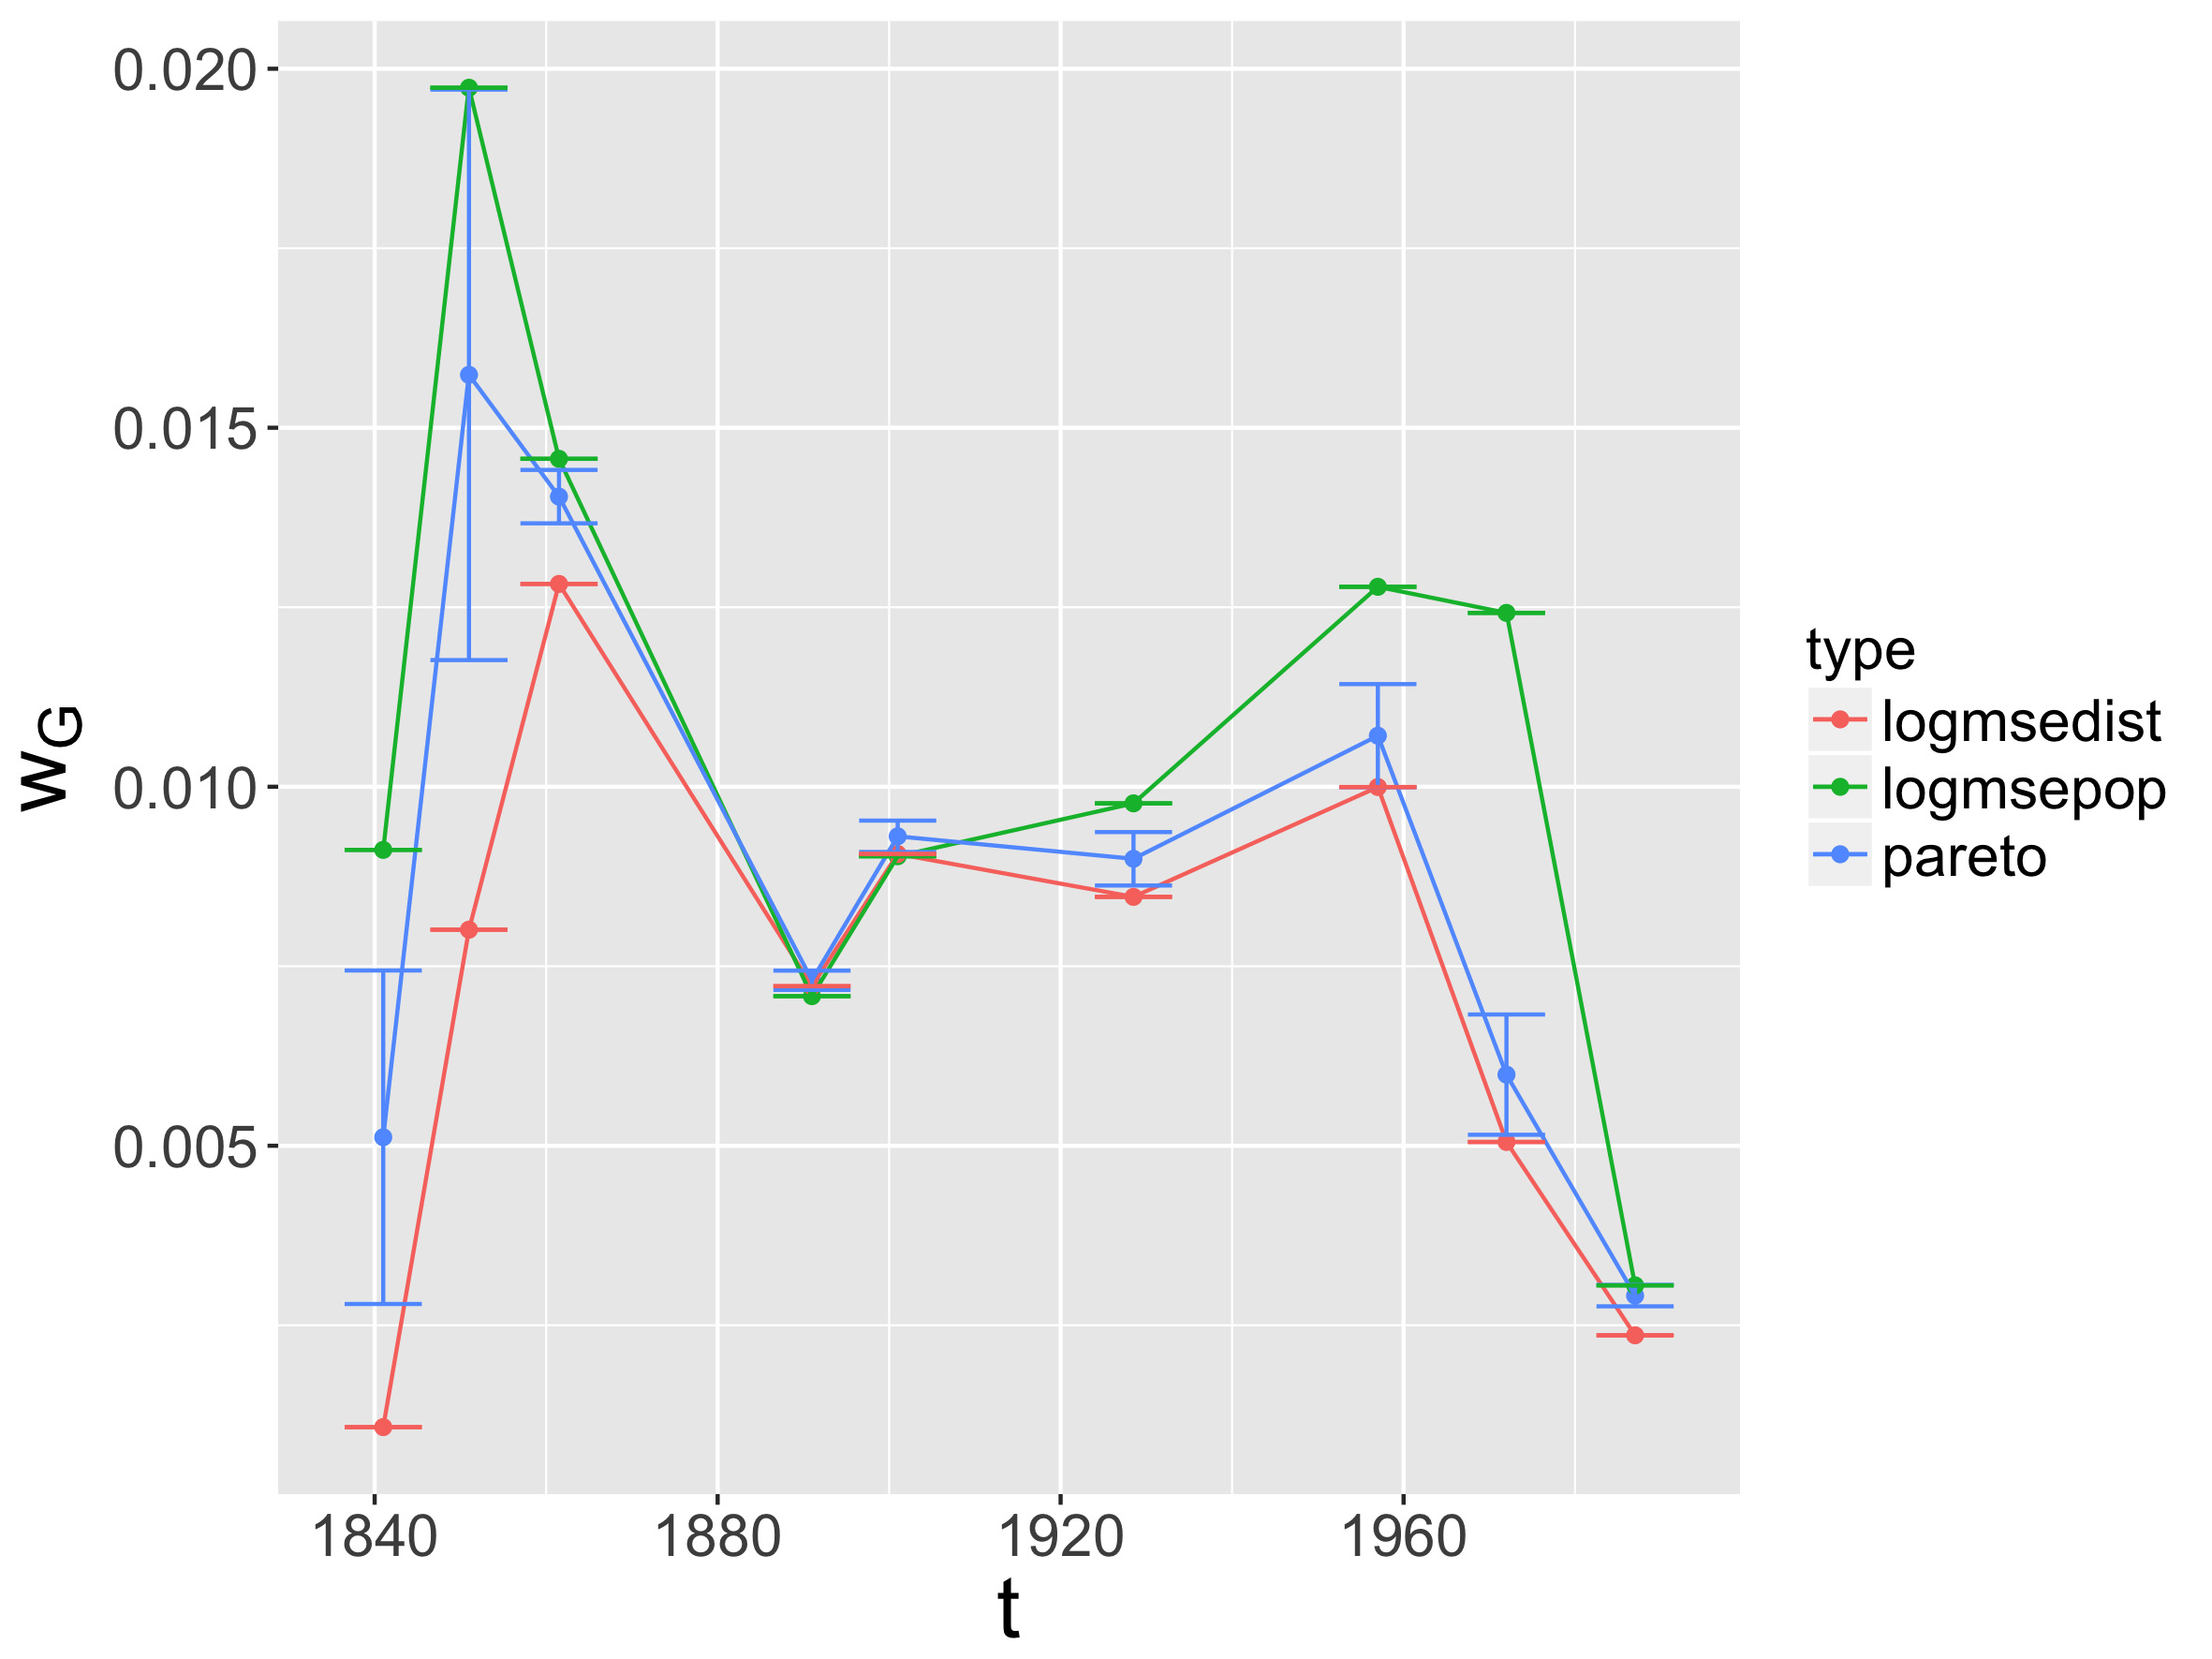
\includegraphics[width=0.32\linewidth]{Figures/MacroCoEvol/param_gravityWeight_filt1}
	%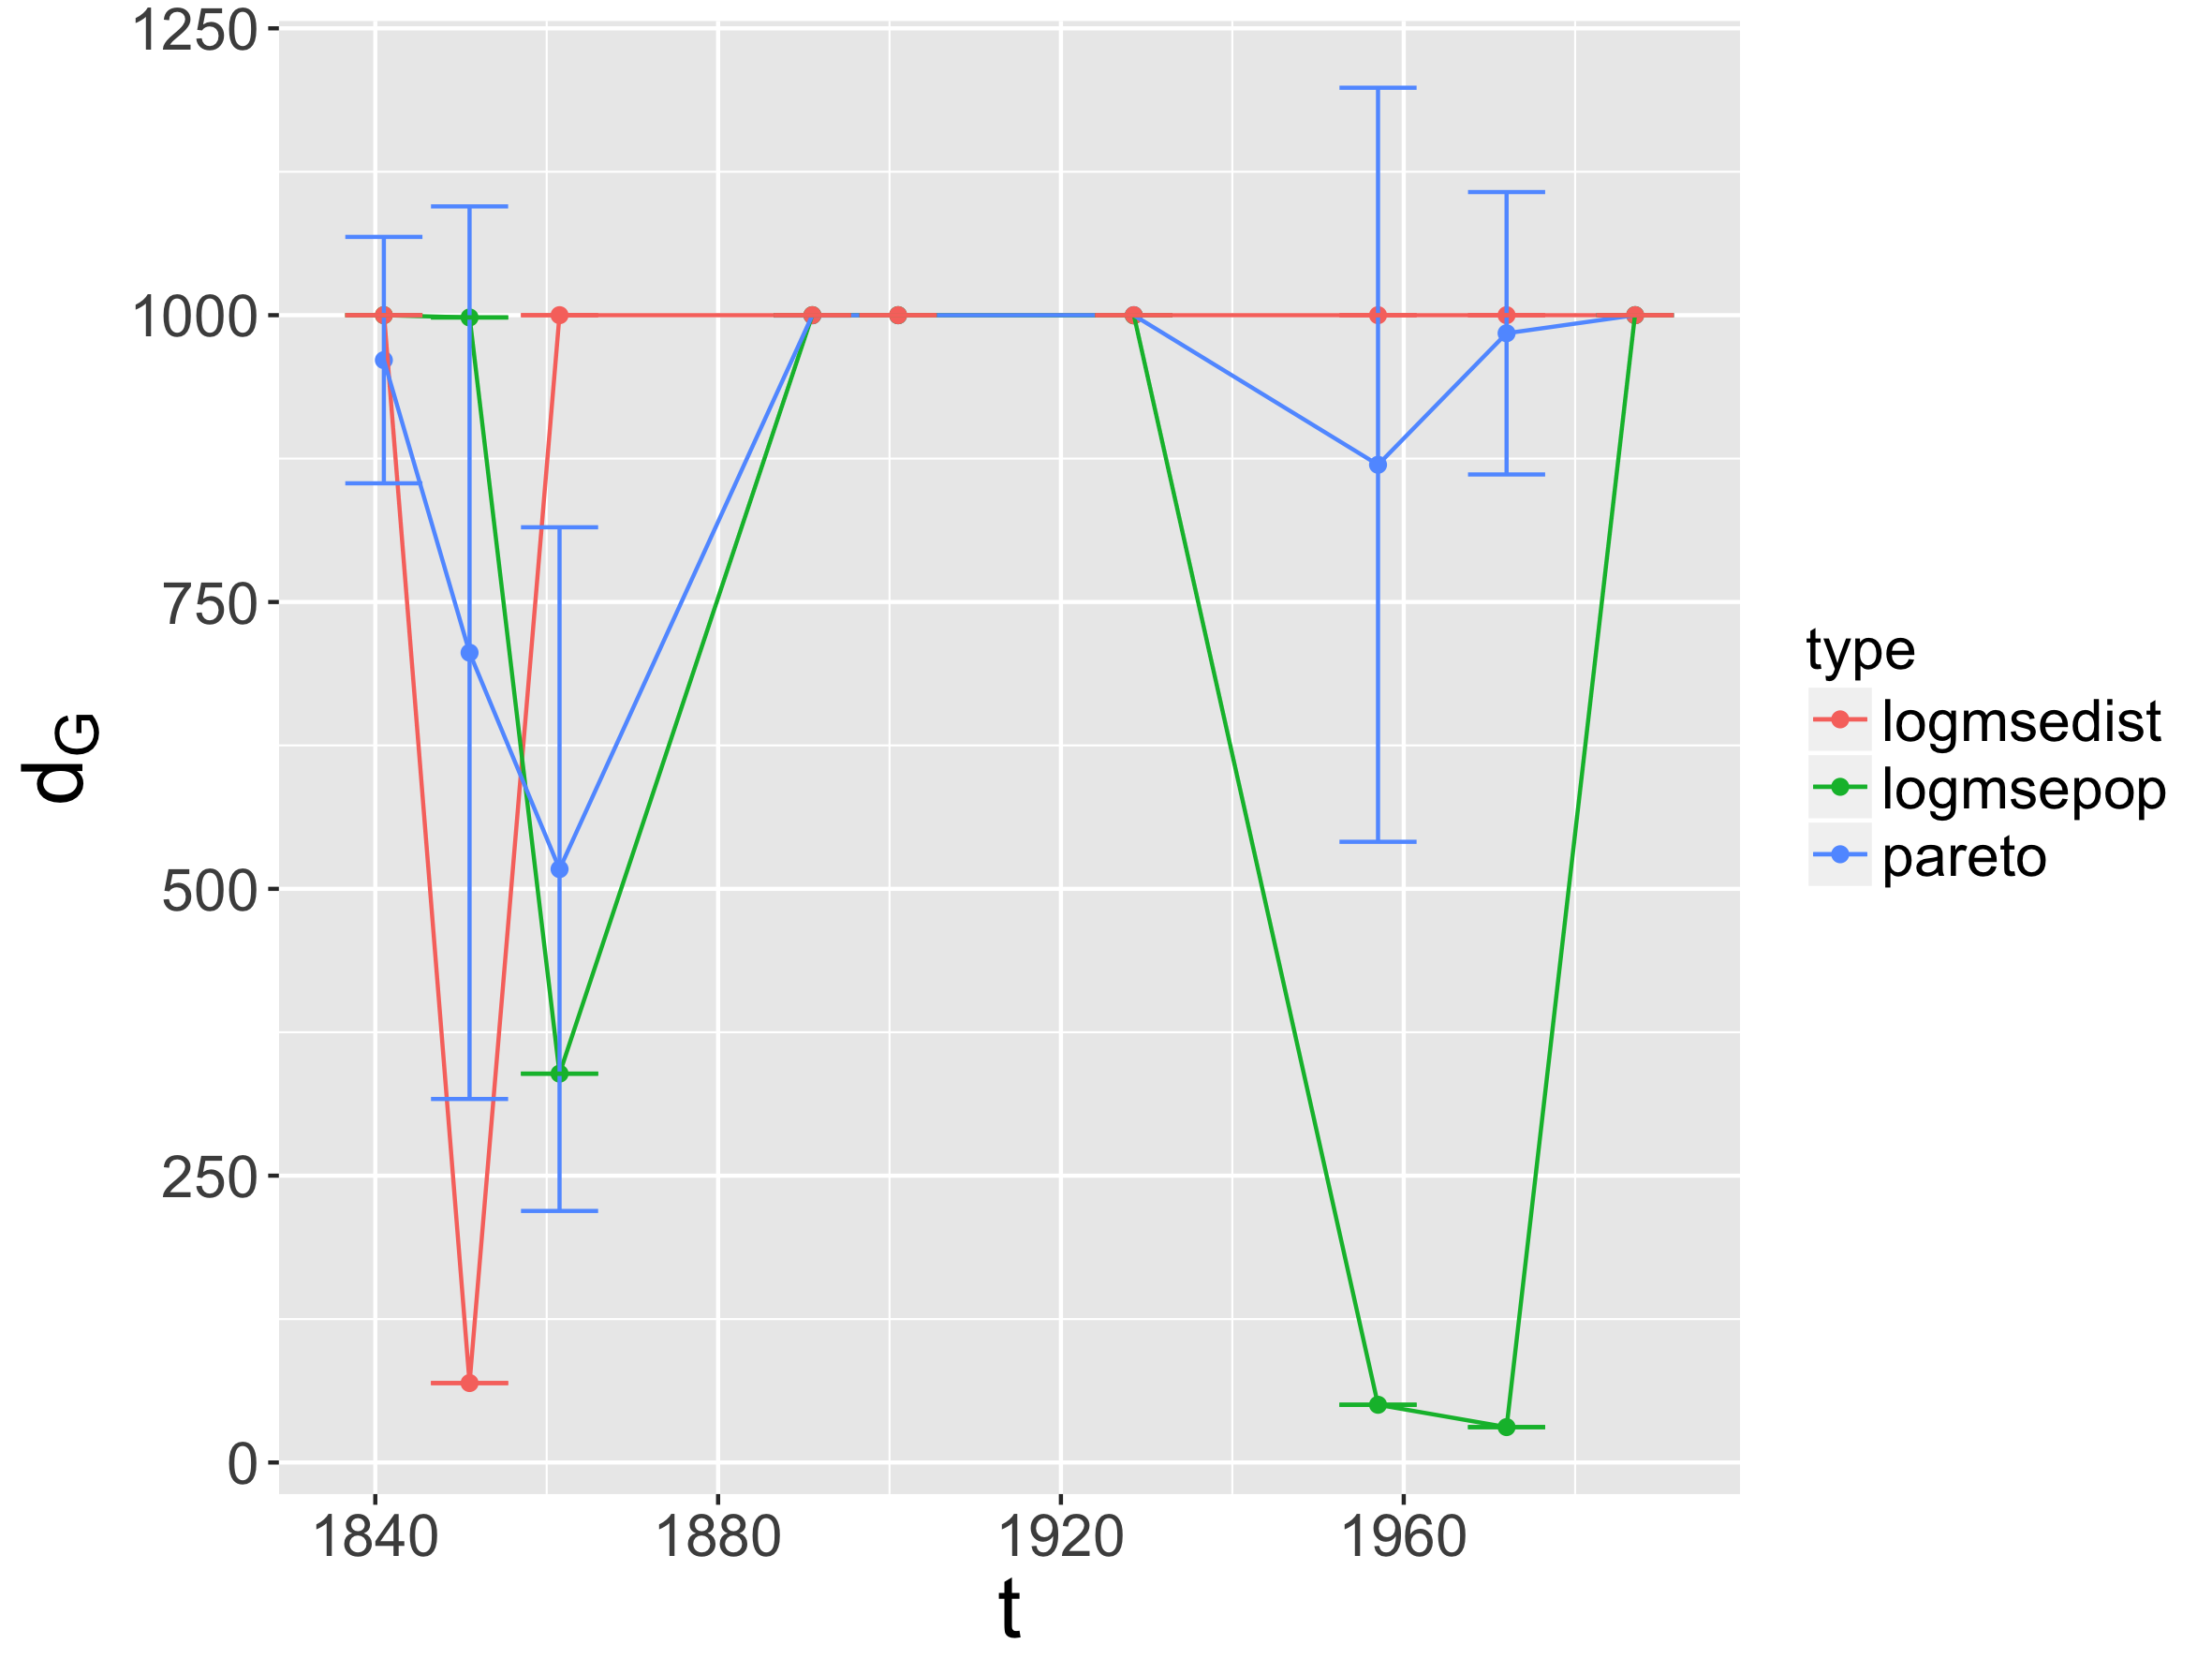
\includegraphics[width=0.32\linewidth]{Figures/MacroCoEvol/param_gravityDecay_filt1}
	%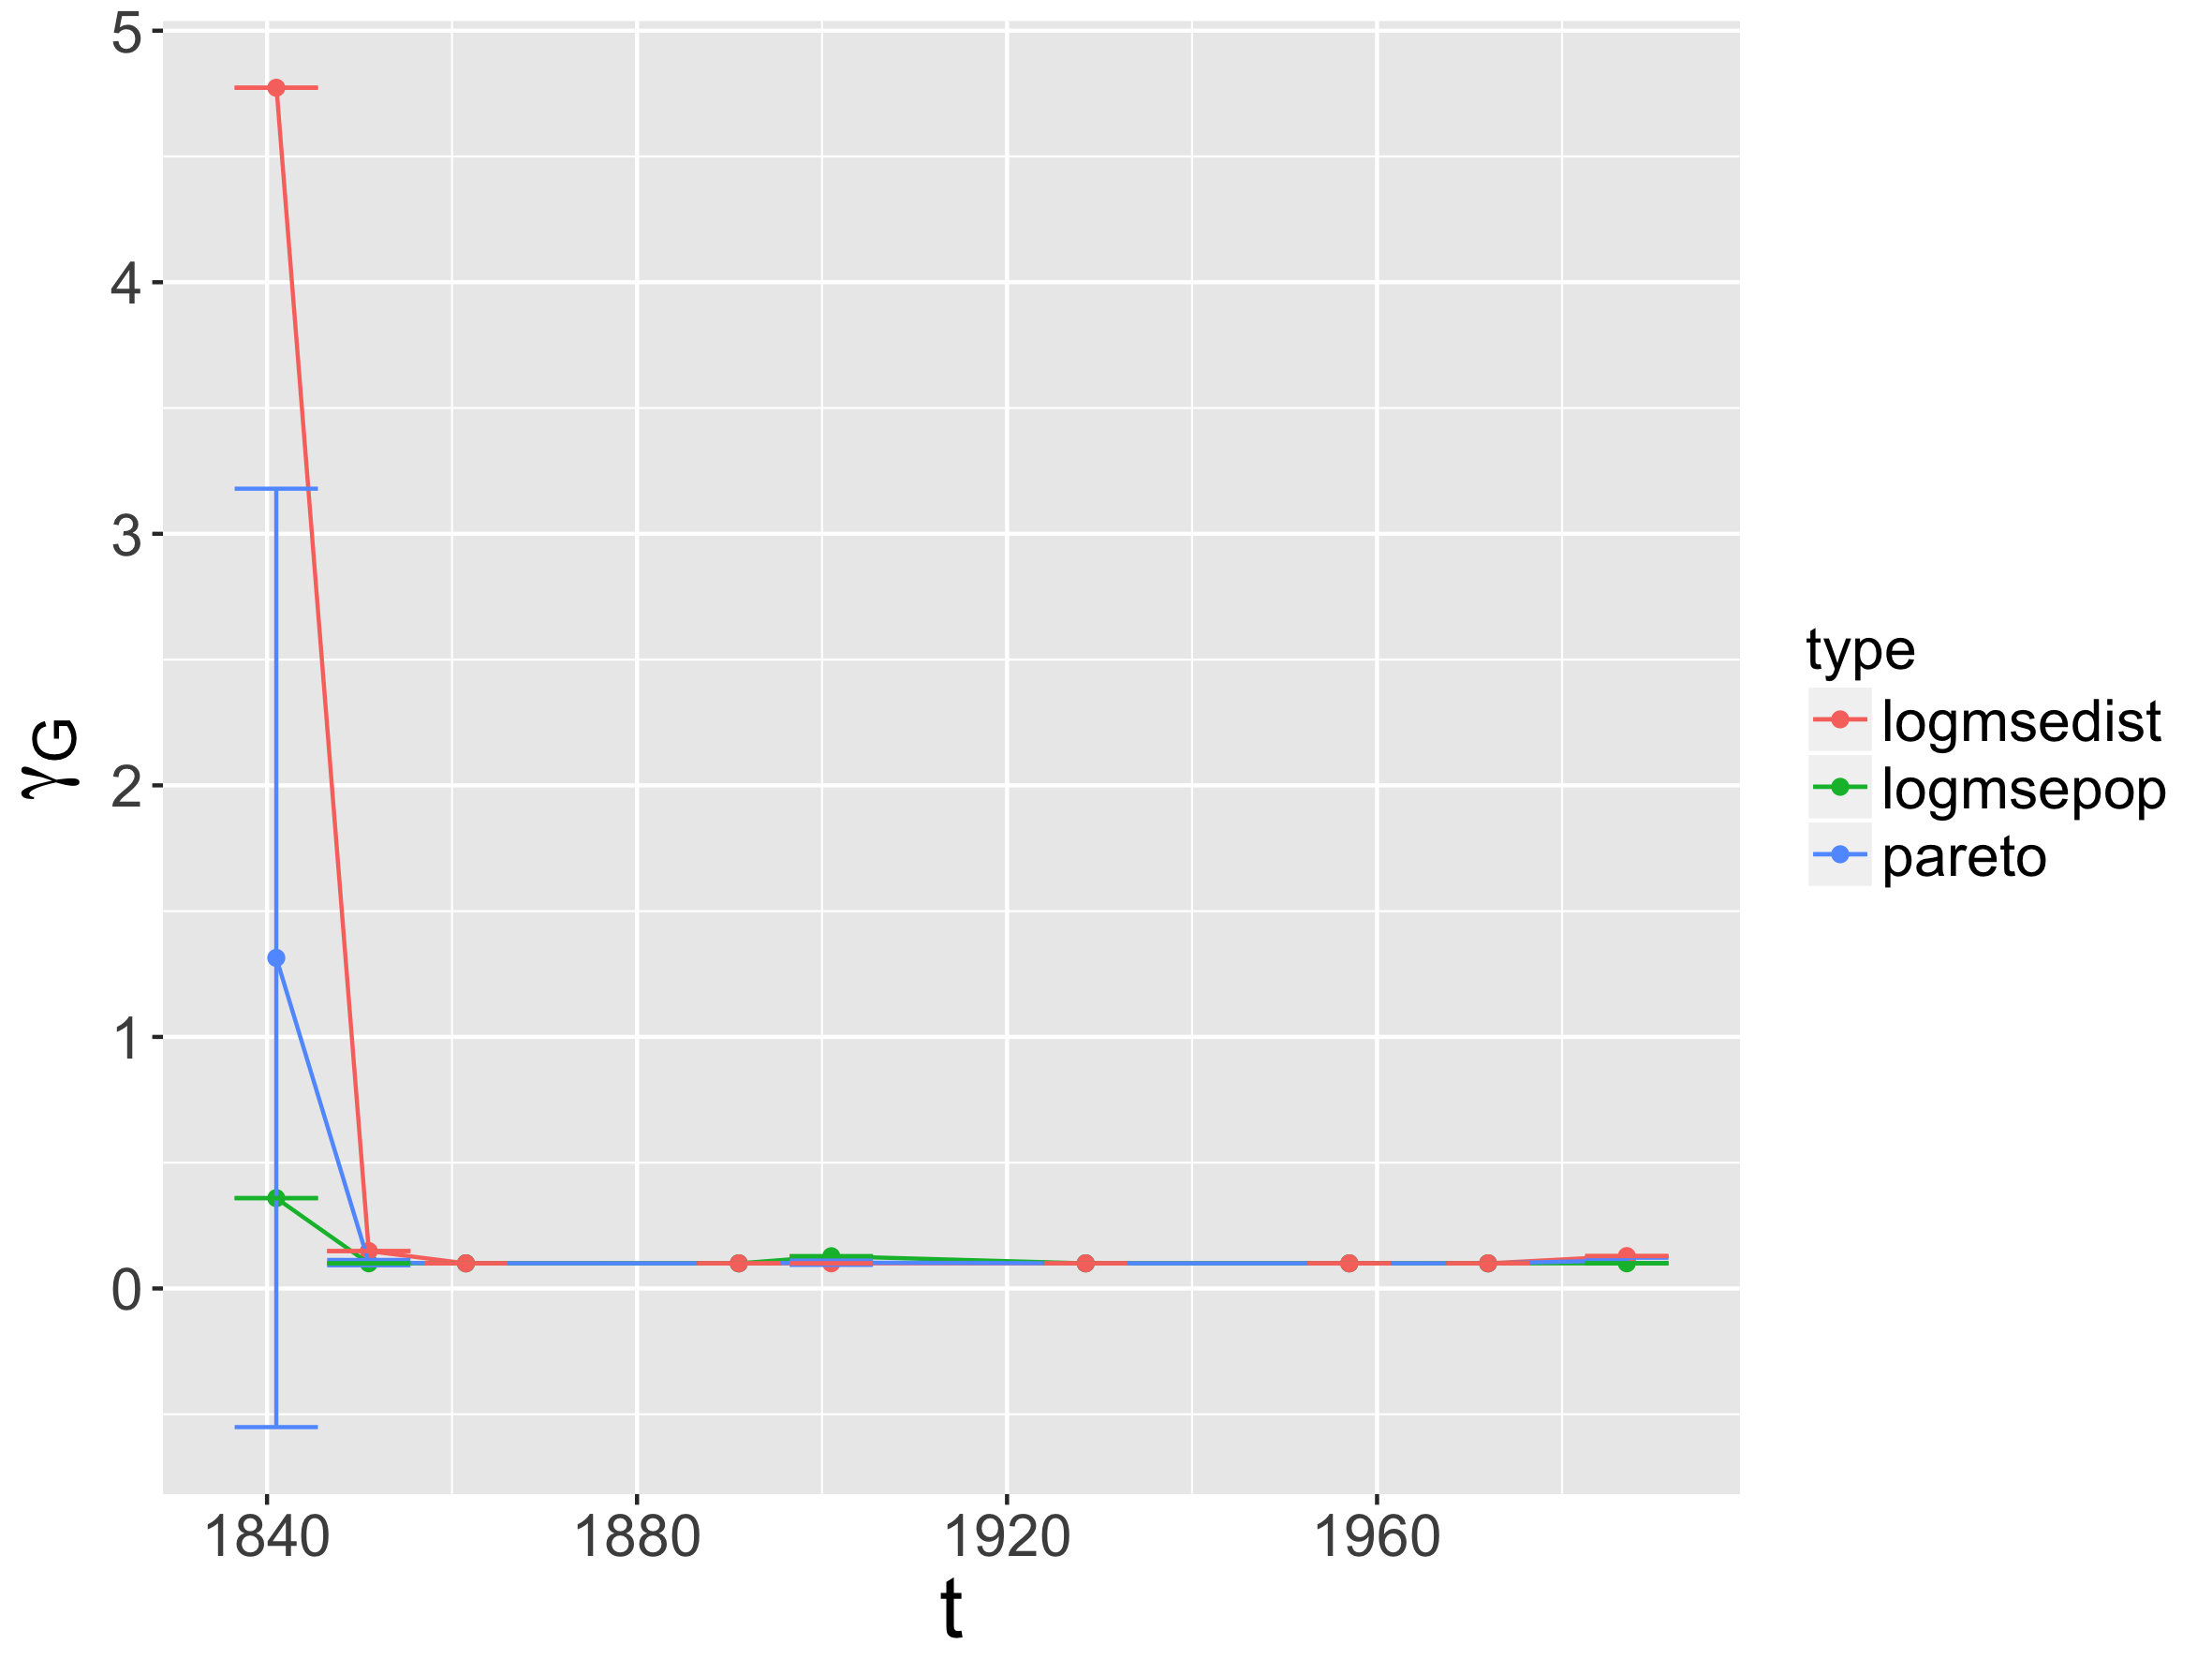
\includegraphics[width=0.32\linewidth]{Figures/MacroCoEvol/param_gravityGamma_filt1}\\
	%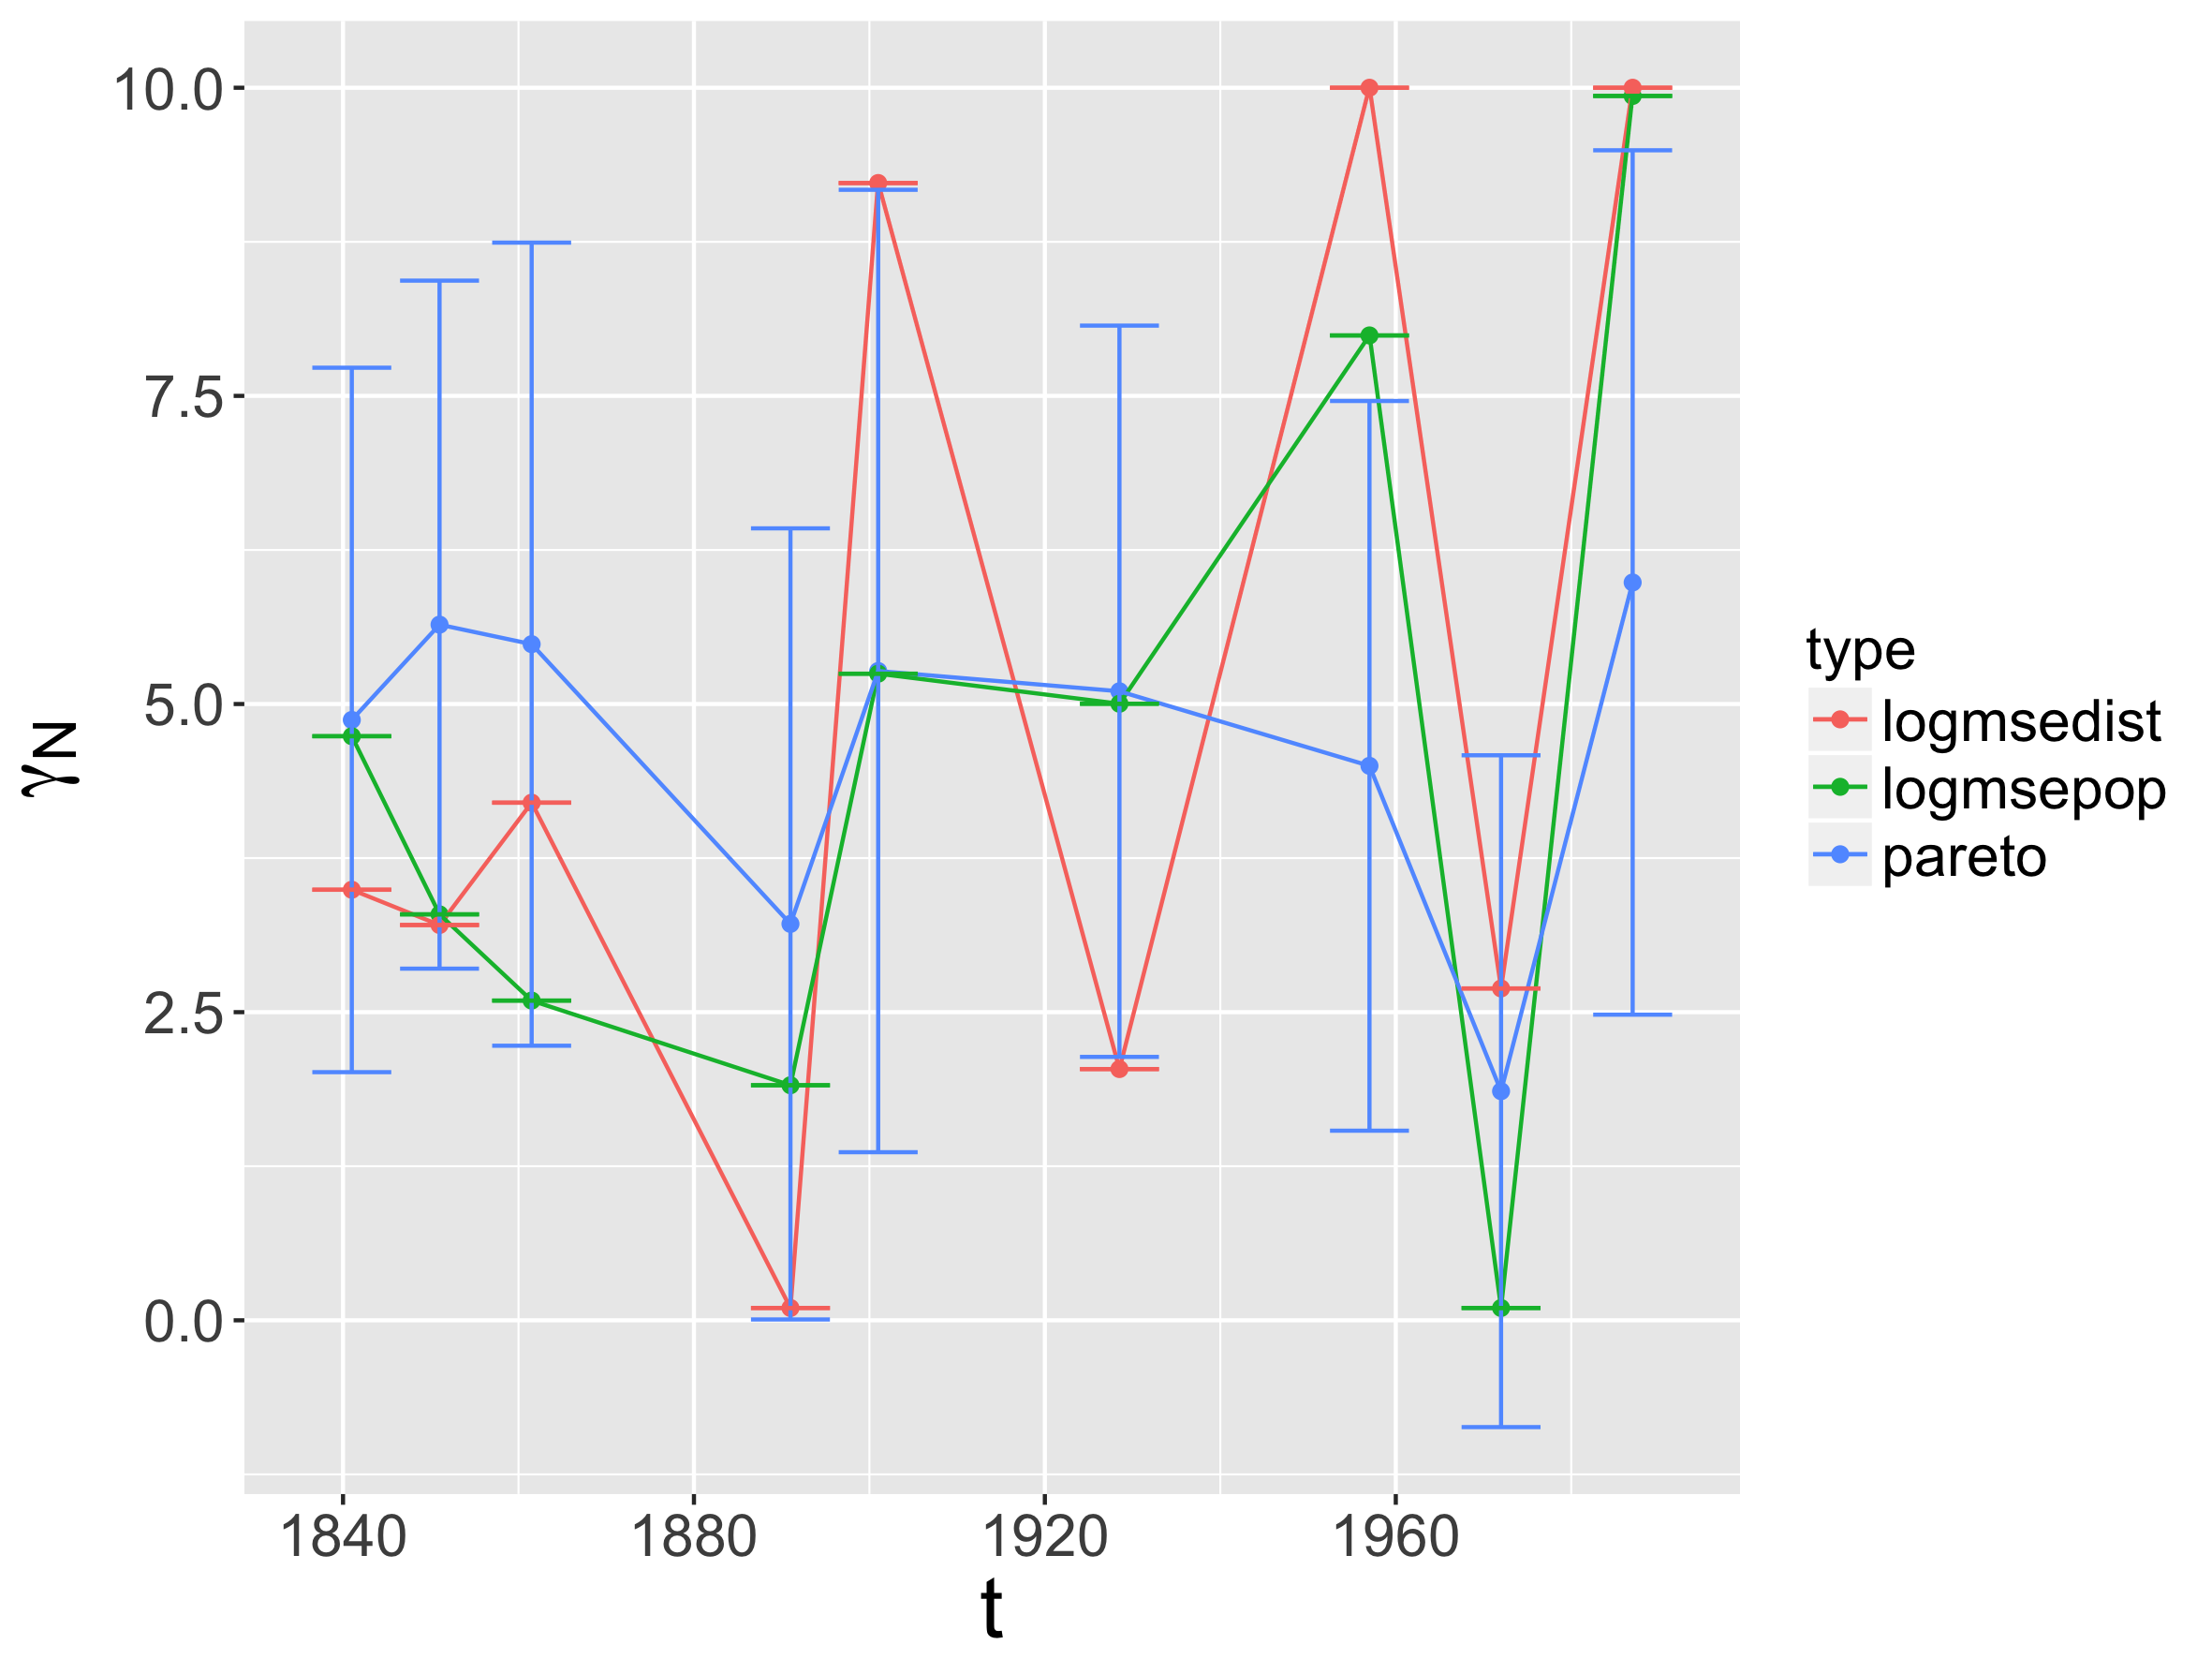
\includegraphics[width=0.32\linewidth]{Figures/MacroCoEvol/param_nwExponent_filt1}
	%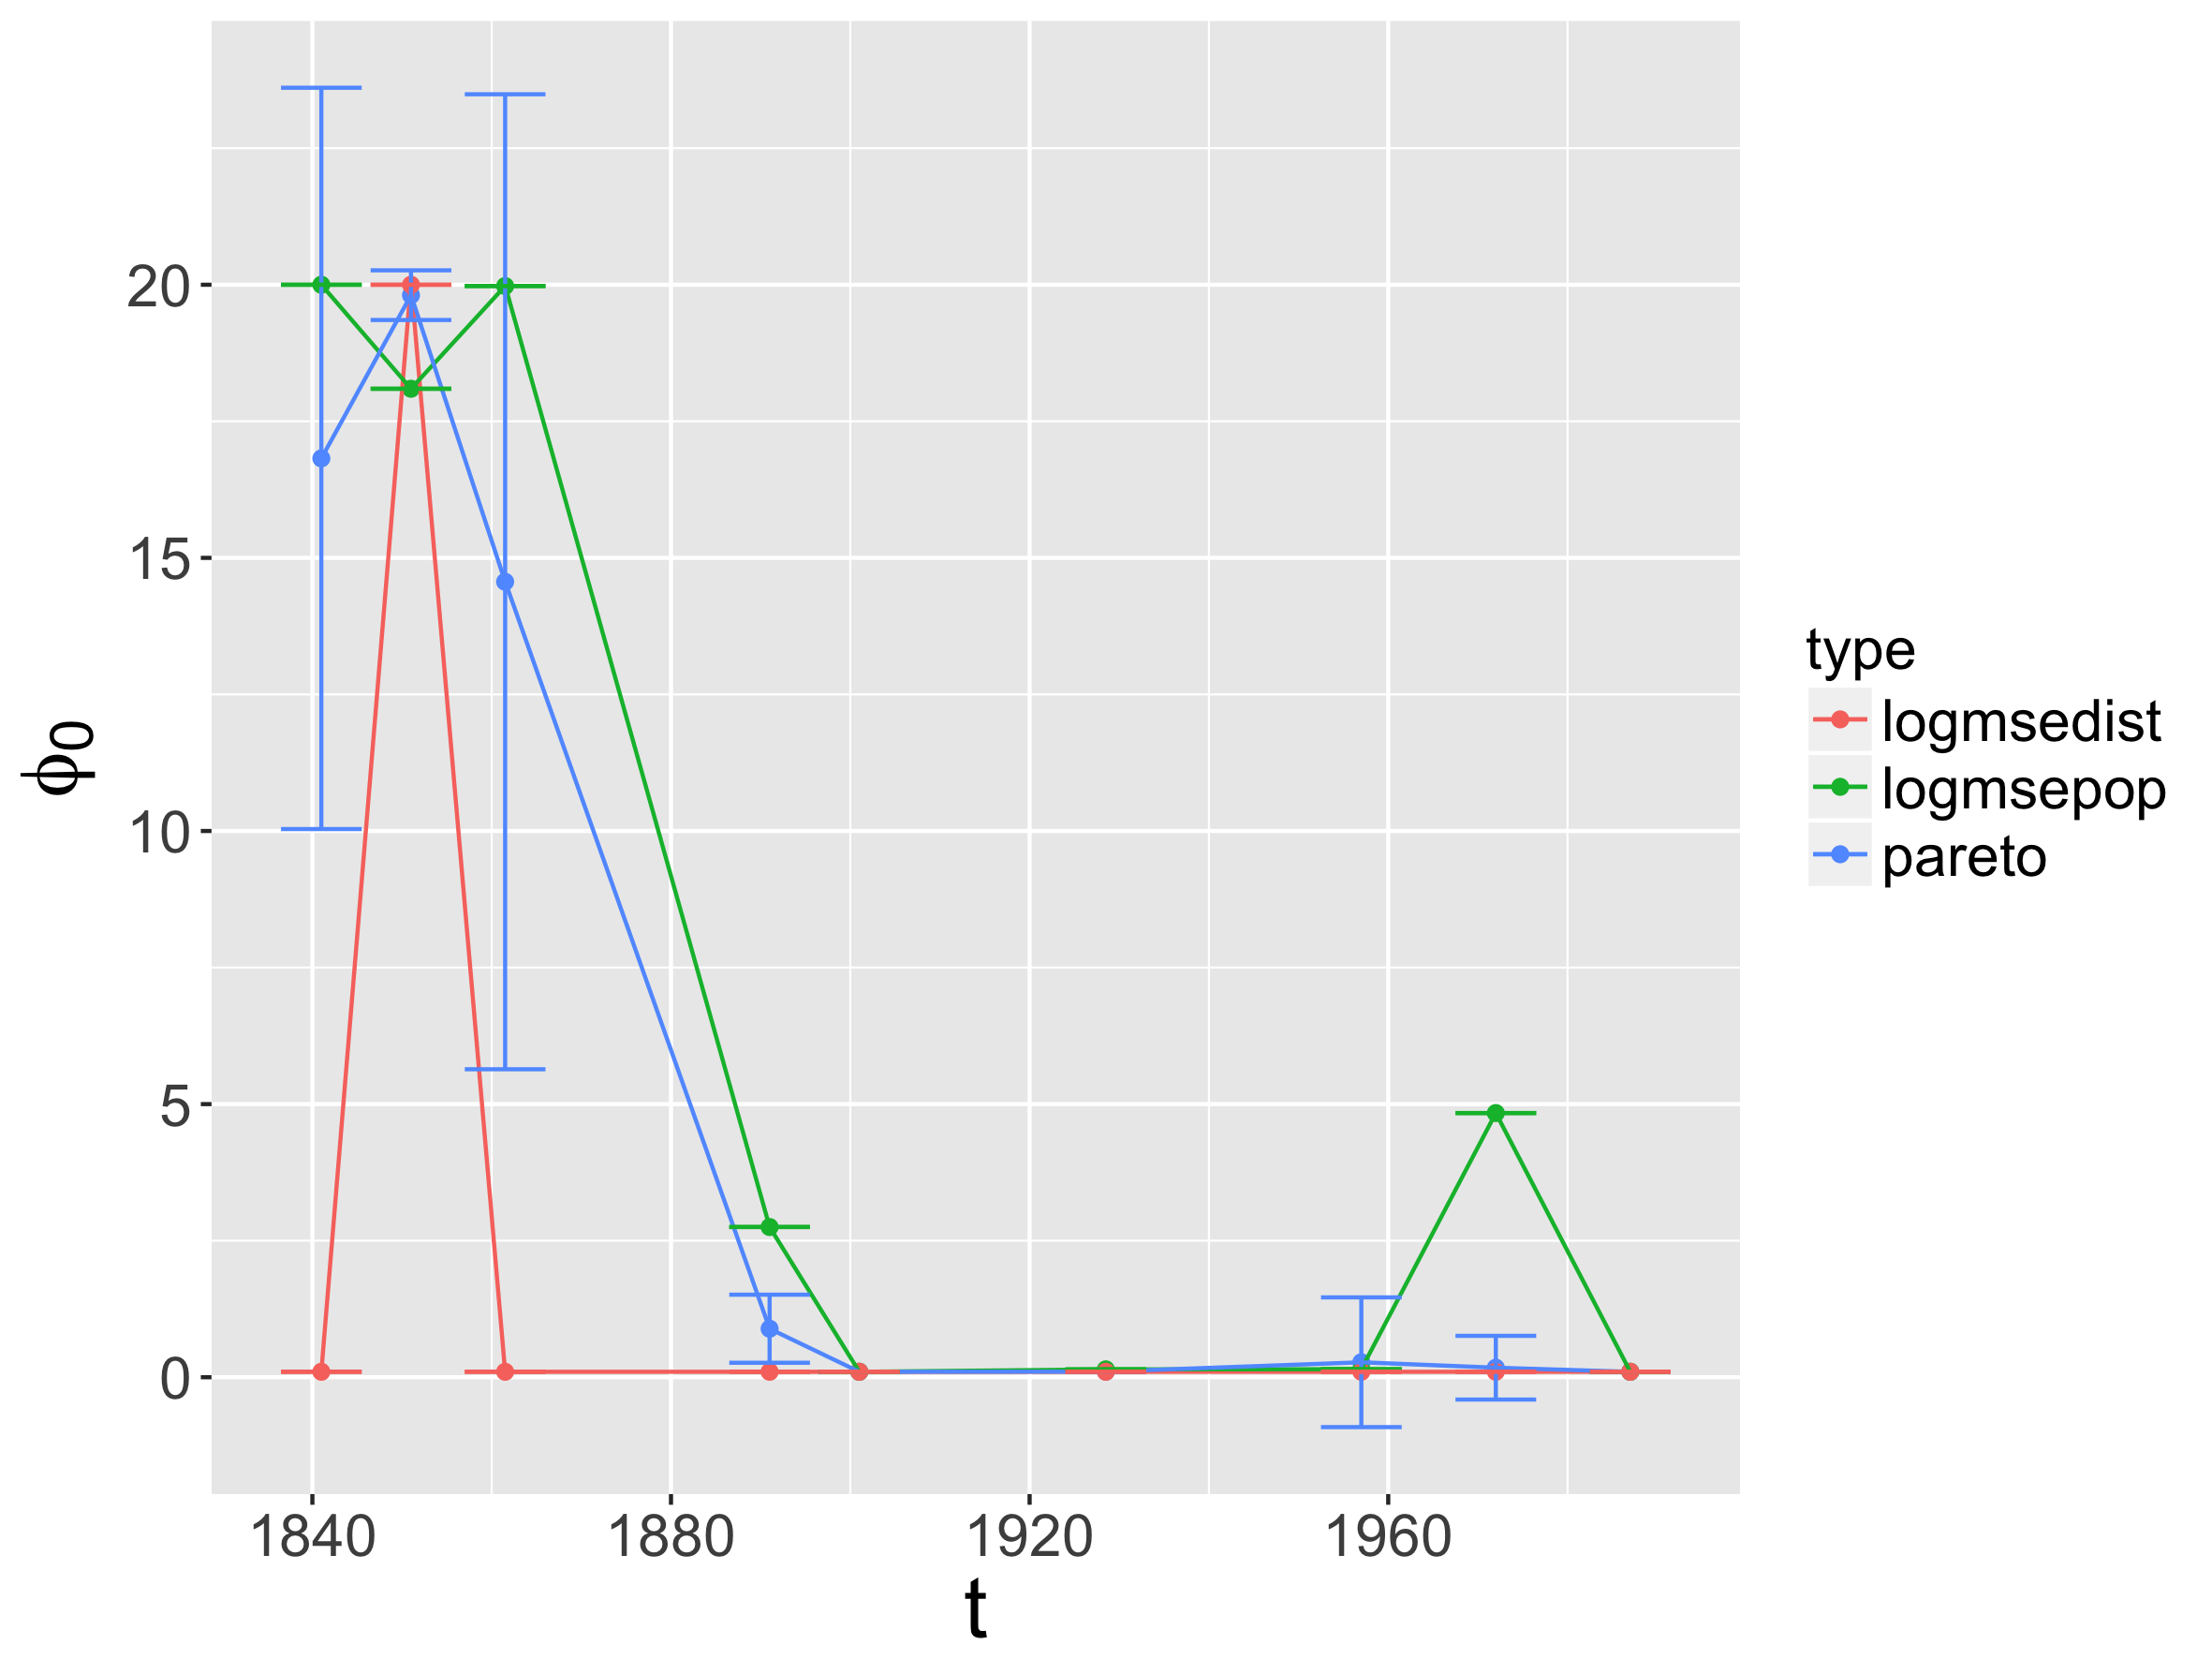
\includegraphics[width=0.32\linewidth]{Figures/MacroCoEvol/param_nwThreshold_filt1}
	%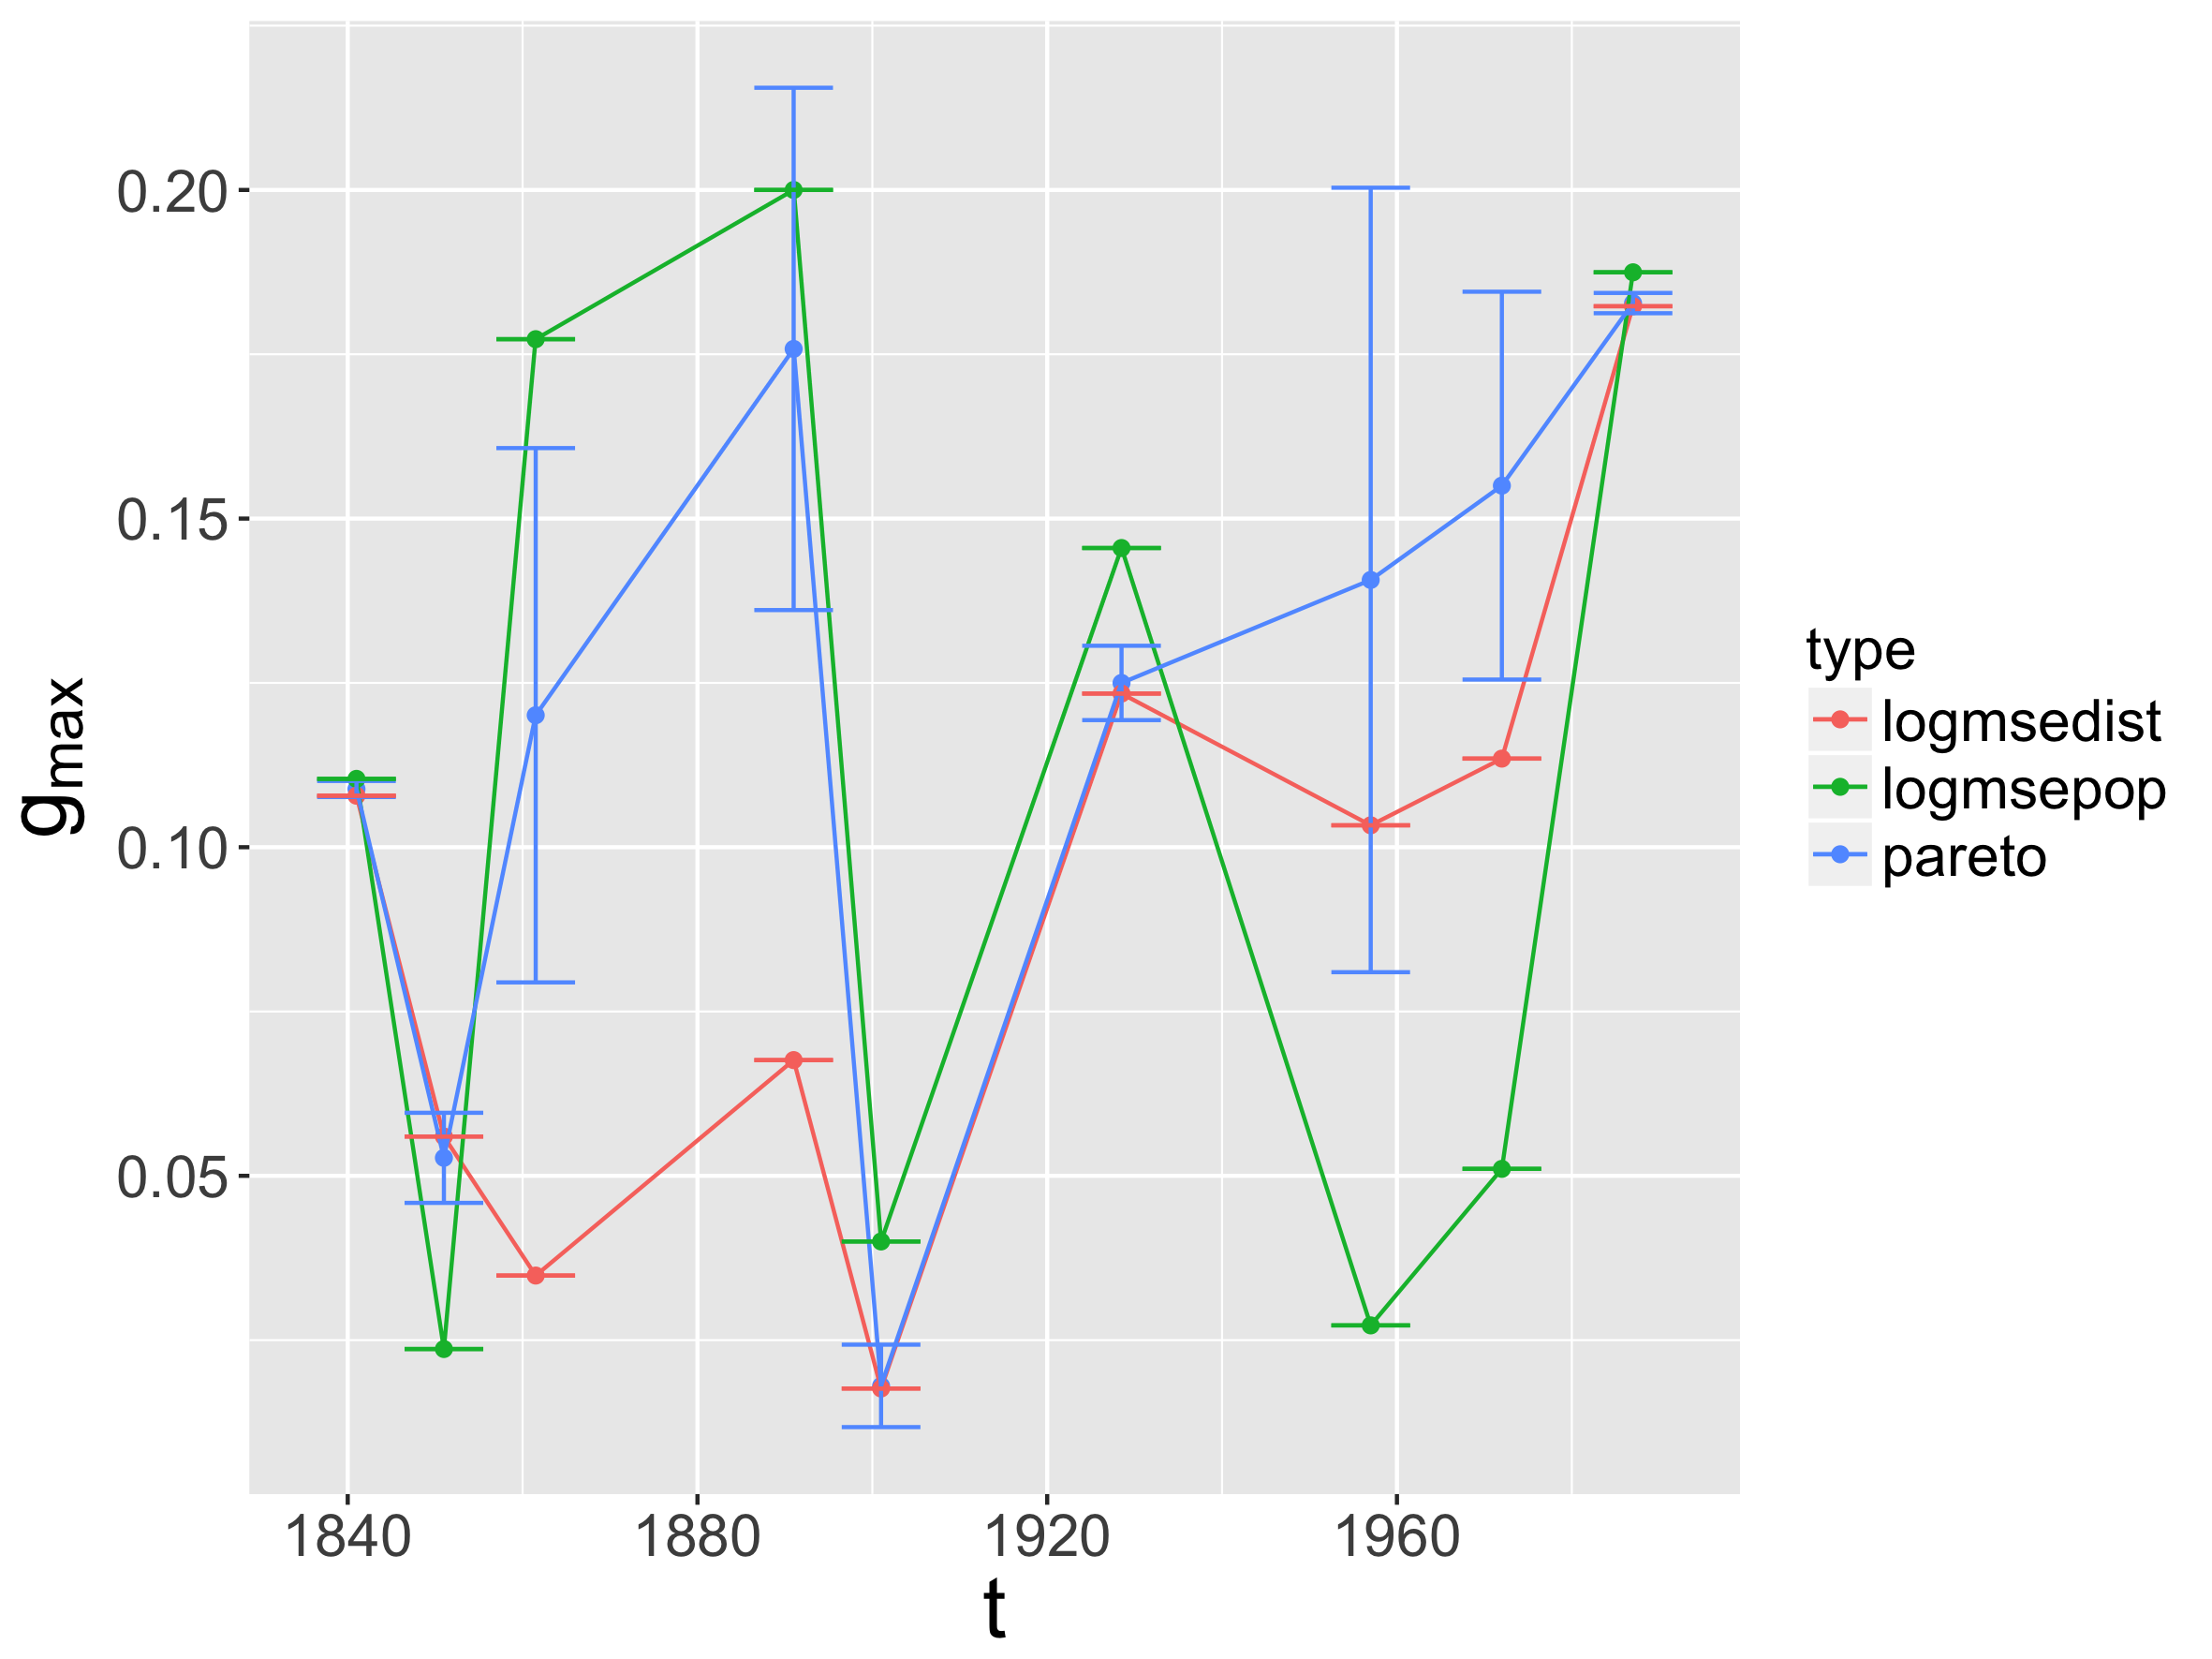
\includegraphics[width=0.32\linewidth]{Figures/MacroCoEvol/param_nwGmax_filt1}
	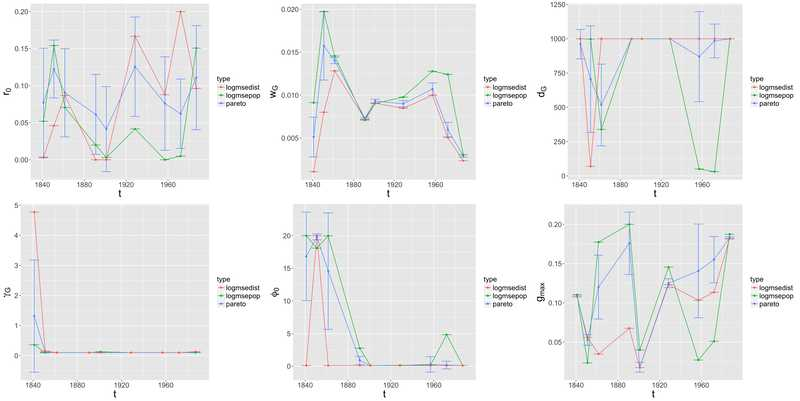
\includegraphics[width=\linewidth]{Figures/Final/6-2-3-fig-macrocoevol-parameters.jpg}
	\caption[Evolution of optimal parameters][Évolution des paramètres calibrés]{\label{fig:macrocoevol:parameters}}{\textbf{Evolution temporelle des paramètres optimaux.} Dans l'ordre de gauche à droite et de haut en bas, valeurs des paramètres $(r_0,w_G,d_G,\gamma_G,\phi_0,g_{max})$, respectivement pour l'ensemble du front de Pareto (bleu), pour le point optimal au sens de la distance (rouge) et pour le point optimal au sens de la population (vert).\label{fig:macrocoevol:parameters}}
\end{figure}
%%%%%%%%%%%%%%%%%%%








\subsubsection{Physical network}{Modèle avec réseau physique}


Nous esquissons à présent les contours d'une spécification du modèle avec réseau physique, qui correspondrait en un sens à un modèle hybride combinant plusieurs échelles. L'idée d'une telle spécification serait d'une part d'étudier l'écart de trajectoire par rapport au réseau abstrait, c'est-à-dire quantifier l'importance des économies d'échelles (liées aux tronçons communs) et de la congestion, ainsi que les possibles compromis à effectuer liés à la spatialisation du réseau, et d'autre part d'étudier dans quelle mesure il est possible de reproduire des réseaux réalistes en comparaison à des modèles autonomes de croissance de réseau par exemple. Ces questions sont traitées à une autre échelle et pour d'autres spécifications ontologiques au chapitre~\ref{ch:mesocoevolution}. 

Une telle spécification rejoint la logique de \cite{li2014modeling}, qui modélise la co-évolution des couloirs de transport et de la croissance des principaux pôles à une échelle régionale.

Le réseau physique que nous implémentons cherche à satisfaire un critère de gain de temps local. Plus précisément, on suppose un auto-renforcement à la manière de~\cite{tero2010rules}. Une specification analogue à celle utilisée précédemment suppose une croissance pour chaque lien, donnée également dans une logique d'auto-renforcement par :

\[
d(t+1) = d(t)\cdot \left(1 + g_{max} \cdot \left[\frac{\phi}{\max \phi}\right]^{\gamma_s}\right)
\]

si $\phi$ est le flux dans le lien et $d(t)$ sa distance effective. La specification par seuil utilisée précédemment ne permet en effet pas une bonne convergence dans le temps, notamment par l'émergence de phénomènes d'oscillation locale.

Nous générons un réseau initial aléatoire, en perturbant la position des sommets d'une grille dont une proportion fixée de liens a été supprimée (40\%) et en y reliant les villes au plus court. Les liens ont tous même impédance, puis celle-ci évolue selon l'équation ci-dessus. Un exemple de configuration obtenue par cette spécification est donné en Fig.~\ref{fig:macrocoevolution:slimemould}. Les bonnes propriétés de convergence (stabilisation visuelle de la structure du réseau lors d'expériences restreintes) suggèrent les potentialités offertes par cette spécification, dont l'exploration systématique est hors de notre portée ici.


%%%%%%%%%%%%%%%%%%%%%%
\begin{figure}
	%\includegraphics[width=0.45\linewidth]{Figures/MacroCoEvol/example_slimemould_1_t0}
	%\includegraphics[width=0.45\linewidth]{Figures/MacroCoEvol/example_slimemould_1_tf}
	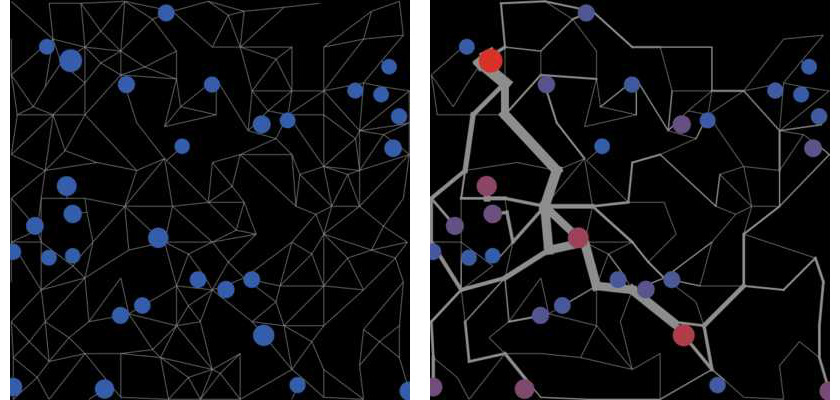
\includegraphics[width=\linewidth]{Figures/Final/6-2-3-fig-macrocoevol-slimemould}
	\caption[Example of self-reinforcing network][Example d'application du modèle macroscopique avec réseau auto-renforçant]{\textbf{Example of configuration obtained with a self-reinforcing network.}\label{fig:macrocoevolution:slimemould}}{\textbf{Example de configuration obtenue avec réseau auto-renforçant.} \textit{(Gauche)} Configuration initiale aléatoire, capacités égales ; \textit{(Droite)} Configuration finale obtenue après 100 itérations.\label{fig:macrocoevolution:slimemould}}
\end{figure}
%%%%%%%%%%%%%%%%%%%%%%


%%%%%%%%%%%%%%%%%
%% ON HOLD


%\begin{enumerate}
%\item le modèle produit-il des formes de réseau crédibles dans le cas du réseau physique ?
%\item éventuellement si les correlations temporelles sont calculées sur les vrais données, le modèle peut-il être calibré au second ordre (sur les correlations/causalités) ?
%\end{enumerate}


%\comment{\cite{mimeur:tel-01451164} la thèse de Mimeur est un pont intéressant entre géographie et approches éco de Levinson (modèle de croissance type slime mould ?). plus fait des stats spatiales pour lier croissance pop et accessibilité : checker si même résulats quand fera spatio-temp causalities sur réseau ferré et autoroutier et croissance pop. remarque : trucs bizzares, essaie d'expliquer pour petites villes, mais pas approprié, pb du choix de l'échelle, de ce qui est du bruit et du signal - semble tout mélanger : importance du preprocessing et traitement du signal (cf correlations des taux de croissance). Tester effets fixes régions/départements ? fait GWR finalement ?}




\subsubsection{Perspectives}{Perspectives}



\paragraph{Particular trajectories}{Trajectoires particulières}


\bpar{
The role of medium-sized cities on the trajectories of the system can also be examined with the model.
}{
L'étude de trajectoires particulières au sein du système de villes peut permettre de répondre à des questions thématiques spécifiques : par exemple, l'influence des villes moyennes sur la trajectoire globale du système, ou les déterminants d'une plus ou moins bonne ``réussite'' pour ce type de profil. Dans le cas de l'application à un système réel, la cartographie des déviations au modèle dans le temps peut suggérer des particularités régionales.
}




\paragraph{Comparison of Urban Systems}{Comparaison de systèmes urbains}


\bpar{
Finally, a comparison between the urban systems in different geographical and political contexts and at different scales should unveil implications of planning on the interactions between networks and cities, for example by comparing the rather bottom-up growth of the French railway network to the top-down state-planned French highway and Chinese HSR networks.
}{
Nous nous attendons finalement également à pouvoir par l'intermédiaire de ce modèle comparer des systèmes urbains dans des contextes géographiques et politiques différents, ainsi qu'à différentes échelles. Cela devrait permettre de révéler les implications des actions de planification sur les interactions entre réseaux et territoires. Par exemple, le réseau ferré français a émergé par l'intermédiaire de multiples opérateurs, au contraire du réseau ferré à grande vitesse Chinois, pour lequel un développement précis pourrait être envisagé.
}





\stars





